%!TEX root=../../main.tex


\begin{doublespace}

\chapter{Introduction to data}
\label{introductionToData}


Advances in science are almost always the result of a dynamic balance between theory and observation. These observations -- collected from the likes of field notes, surveys, and experiments -- form the backbone empirical research and are called \term{data}. Statistics is the study of how to best collect, analyze, and draw conclusions from data. Statistics is an integral part of the components of the scientific method:  
\begin{enumerate}
\setlength{\itemsep}{0mm}
\item Identify a question or problem.
\item Collect relevant data on the topic.
\item Analyze the data.
\item Form a conclusion.
\end{enumerate}
Statistics as a subject focuses on making stages 2-4 objective, rigorous, and efficient. That~is, statistics has three primary components: How can data best be collected? How should it be analyzed? What can be inferred from the analysis?  

This chapter provides a brief introduction to the principles of data collection and introduces some simple numerical and graphical summaries of data that will be used in the rest of the text.  The examples are drawn from recent studies in medicine and biology and illustrate the important role statistics plays in medicine and biology.  The chapter also serves as a brief review for readers already familiar with introductory statistics.


\section[Case study]{Case study: preventing peanut allergies}
\label{leapCaseStudy}

\index{data!LEAP|(}

Section~\ref{leapCaseStudy} introduces an important problem in medicine: evaluating the effect of a strategy for treating a disease or medical condition. Terms in this section, and indeed much of this chapter, will be revisited later in more detail.

The proportion of young children in Western countries with peanut allergies has doubled in the last 10 years. Previous research suggests that exposing infants to peanut-based foods, rather than excluding such foods from their diets, may be an effective strategy for preventing the development of peanut allergies. This section describes an experiment (a clinical trial, in the terminology of medical research) designed to address the following research question: Does early exposure to peanut products reduce the probability that a child will develop peanut allergies? 

The "Learning Early about Peanut Allergy" (LEAP) study was reported in the New England Journal of Medicine in 2015.\footnote{Du Toit, George, et al. Randomized trial of peanut consumption in infants at risk for peanut allergy. New England Journal of Medicine 372.9 (2015): 803-813.} The study team enrolled children in the United Kingdom between 2006 and 2009, selecting 640 infants with eczema, egg allergy, or both. Each child was randomly assigned to the treatment group (peanut consumption) or the control group (peanut avoidance); children in the treatment group were fed at least 6 grams of peanut protein daily until 5 years of age, while children in the control group were to avoid consuming peanut protein until 5 years of age. 

At 5 years of age, each child was tested for peanut allergy using an oral food challenge (OFC): 5 grams of peanut protein in a single dose. Children had been previously been tested for peanut allergy through a skin test, conducted at the time of study entry; the main analysis presented in the paper was based on the 530 children with a negative skin test result. Of these children, 263 were assigned to "Peanut Avoidance" and 267 to "Peanut Consumption." The outcome at 5 years was reported as either "Fail OFC" (allergic reaction) or "Pass OFC" (no allergic reaction). 

Table \ref{leapStudyResultsDF} shows the participant study ID number, treatment assignment, and OFC outcome for 5 children. All five of these children passed the food challenge. 
 
% latex table generated in R 3.1.1 by xtable 1.7-4 package
% Mon Sep 28 09:14:28 2015

\begin{table}[ht]
\centering
\begin{tabular}{lll}
  \hline
participant.ID & treatment.group & overall.V60.outcome \\ 
  \hline
LEAP\_100522 & Peanut Consumption & PASS OFC \\ 
  LEAP\_103358 & Peanut Consumption & PASS OFC \\ 
  LEAP\_105069 & Peanut Avoidance & PASS OFC \\ 
  LEAP\_994047 & Peanut Avoidance & PASS OFC \\ 
  LEAP\_997608 & Peanut Consumption & PASS OFC \\ 
   \hline
\end{tabular}
\caption{Results for five children from the peanut study.}
\label{leapStudyResultsDF}
\end{table}

%print(xtable(LEAP[c(1,2,3,529, 530),c("participant.ID", "treatment.group", "overall.V60.outcome")]),include.rownames=FALSE)

When looking for patterns in data, summary tables are generally more helpful than individual participant listings. Table~\ref{leapStudyResults} shows outcomes grouped by treatment group and the result of the OFC test. From this table, it is possible to compute some simple summary statistics. 

% latex table generated in R 3.1.1 by xtable 1.7-4 package
% Thu Jul 16 07:12:04 2015
\begin{table}[ht]
\centering
\begin{tabular}{rrrr}
  \hline
 & FAIL OFC & PASS OFC & Sum \\ 
  \hline
Peanut Avoidance & 36 & 227 & 263 \\ 
  Peanut Consumption & 5 & 262 & 267 \\ 
  Sum & 41 & 489 & 530 \\ 
   \hline
\end{tabular}
\caption{LEAP Study Results} 
\label{leapStudyResults}
\end{table}
%library(xtable); outcome.table = addmargins(table(LEAP$treatment.group, LEAP$overall.V60.outcome)); xtable(outcome.table, digits = 0, caption = "LEAP Study Results", caption  = "leapStudyResults")


A \term{summary statistic} is a single number summarizing a large amount of data.\footnote{Formally, a summary statistic is a value computed from the data.} In the Peanut Avoidance group, the proportion of participants failing the food challenge at 5 years of age is 36/263 = 0.137 (13.7\%); in the Peanut Consumption intervention, the proportion failing is 5/267 = 0.019 (1.9\%). The difference between these two proportions, 11.8\%, is a summary statistic describing the extent to which these two proportions differ. A second summary statistic, the ratio of the two proportions, 0.137/0.019 = 7.31, indicates that the proportion failing in the Avoidance group is more than 7 times that of the Consumption group.   
	
The summary statistics for the LEAP study highlight an important point -- the results of a study can sometimes be surprising.  A parent of a child already known to be allergic to eggs might be justifiably skeptical about feeding peanut butter to their child.  The LEAP study suggests that, at least for children similar to those enrolled in the study, the benefits of early exposure might be substantial. 

There are important aspects of the study to be cautious about.  This study was conducted in the United Kingdom at a single site of pediatric care; it is not clear that results in children from that site can be generalized to other countries or cultures. The results also raise an important statistical issue: does the study provide definitive evidence that peanut consumption is beneficial? In other words, is the 11.8\% difference between the two groups larger than one would expect by chance variation alone? 

Suppose a coin is flipped 100 times. While the chance a coin lands heads in any given coin flip is 50\%, observing exactly 50 heads is unlikely; instead, the coin may land heads 43 times, 51 times, 59 times, etc. This type of fluctuation is part of almost any experiment or study. It may well be possible that the 11.8\% difference in the peanut allergy study is only due to this natural variation, and that the two interventions are actually equally effective. However, the larger the difference observed (for a particular study size), the less credible it is that the difference is due to chance alone. If out of 100 flips, a coin landed heads only 5 times, it would be reasonable to doubt that the outcome was due to chance; perhaps the coin is weighted so that tails are more likely to occur.

For the LEAP study, the 11.8\% difference is indeed larger than that expected by chance alone, suggesting that peanut consumption is the more effective intervention for preventing subsequent allergies. The material on hypothesis testing in later chapters will provide the statistical tools to confirm that the result of the study is unlikely if the two interventions had been equally effective.

\index{data!LEAP|)}


\section{Data basics}
\label{dataBasics}

Effective presentation and description of data is a first step in most analyses. This section introduces a structure for organizing data and some terminology that will be used throughout this book.


\subsection{Observations, variables, and data matrices}
\label{frogDataExample}

\index{data!frog|(}
This section describes data used in a study published in the \textit{Journal of Evolutionary Biology} about maternal investment at differing altitudes, conducted in a frog species endemic to the Tibetan Plateau (\textit{Rana kukunoris}).\footnote{ Chen, W., et al. Maternal investment increases with altitude in a frog on the Tibetan Plateau. Journal of evolutionary biology 26.12 (2013): 2710-2715.} Reproduction is a costly process for females, necessitating a trade-off between individual egg size and total number of eggs produced. Researchers collected measurements on egg clutches found at breeding ponds across 11 study sites; for 5 sites, they also collected data on individual female frogs.

% latex table generated in R 3.1.1 by xtable 1.7-4 package
% Fri Jul 17 09:47:19 2015
\begin{table}[ht]
\centering
\begin{tabular}{rlrrrrr}
  \hline
 & altitude & latitude & egg.size & clutch.size & clutch.volume & body.size \\ 
  \hline
1 & 3,462.00 & 34.82 & 1.95 & 181.97 & 177.83 & 3.63 \\ 
  2 & 3,462.00 & 34.82 & 1.95 & 269.15 & 257.04 & 3.63 \\ 
  3 & 3,462.00 & 34.82 & 1.95 & 158.49 & 151.36 & 3.72 \\ 
  150 & 2,597.00 & 34.05 & 2.24 & 537.03 & 776.25 & NA \\ 
   \hline
\end{tabular}
\caption{Frog Study Data Matrix} 
\label{frogDF}
\end{table}
%library(xtable); xtable(frog.altitude[c(1,2,3,529, 530),c( "altitude", "latitude", "egg.size", "clutch.size", "clutch.volume", "body.size")], digits = 2, caption = "Frog Study Data Matrix", label = "frogDF" )

Table~\ref{frogDF} displays rows 1, 2, 3, and 150 of the data from the 431 clutches. The complete set of observations will be referred to as the \data{frog} dataset. Each row in the table corresponds to a single clutch, indicating where the clutch was collected (\var{altitude} and \var{latitude}), \var{egg.size}, \var{clutch.size}, \var{clutch.volume}, and \var{body.size} of the mother when available. "NA" corresponds to a missing value; information on individual females was not collected for that particular site. The columns represent characteristics, called \term{variables}, for each clutch.

For example, the first row represents a clutch collected at altitude 3,462 meters above sea level, latitude 34.82 degrees; the clutch contained an estimated 182 eggs, with individual eggs averaging 1.95 mm in diameter, for a total volume of 177.8 mm$^{3}$. The eggs were laid by a female measuring 3.63 cm long. It is important to understand the definitions of variables, as they are not always obvious. For example, why has \var{clutch.size} not been recorded as whole numbers?  In a given clutch, researchers counted approximately 5 grams' worth of eggs and then estimated the total number of eggs based on the mass of the entire clutch. Definitions of the variables are given in Table~\ref{frogVariables}.\footnote{The data discussed here are in the original scale; in the published paper, some values have been log-transformed.}

\begin{table}[t]
	\centering\small
	\begin{tabular}{lp{10.5cm}}
		\hline
		{\bf variable} & {\bf description} \\
		\hline
		\var{altitude} & Altitude of the study site in meters above sea level \\
		\var{latitude} & Latitude of the study site measured in degrees \\
		\var{egg.size} & Average diameter of an individual egg to the 0.01 mm  \\
		\var{clutch.size} & Estimated number of eggs in clutch\\
		\var{clutch.volume} & Volume of egg clutch in mm$^3$  \\
		\var{body.size} & Length of mother frog in cm \\
		\hline
	\end{tabular}
	\caption{Variables and their descriptions for the \data{frog} dataset.\vspaceB{-3.5mm}}
	\label{frogVariables}
\end{table}

The data in Table~\ref{frogDF} are organized as a \term{data matrix}. Each row of a data matrix corresponds to a unique observational unit, and each column corresponds to a variable. A data matrix for the LEAP study introduced in Section~\ref{leapCaseStudy} is shown in Table~\ref{leapStudyResultsDF} on page~\pageref{leapStudyResultsDF};  the cases are study participants and three variables are shown for each participant. Data matrices are a convenient way to record and store data. If the data are collected for another individual, another row can easily be added; similarly, another column can be added for a new variable.

\index{data!frog|)}


\subsection{Types of variables}
\label{variableTypes}

\index{data!famuss|(}

The Functional polymorphisms Associated with Human Muscle Size and Strength study (FAMuSS), funded by the National Institutes of Health (NIH), measured a variety of demographic, phenotypic, and genetic characteristics for about 1,300 participants.\footnote{Thompson PD, Moyna M, Seip, R, et al., 2004.  Functional Polymorphisms Associated with Human Muscle Size and Strength.  Medicine and Science in Sports and Exercise 36:1132 - 1139} Data from the study has been used in many subsequent studies\footnote{Pescatello L, et al. Highlights from the functional single nucleotide polymorphisms associated with human muscle size and strength or FAMuSS study, BioMed Research International 2013.}, such as one examining the relationship between muscle strength and genotype at a location on the ACTN3 gene.\footnote{Clarkson P, et al., Journal of Applied Physiology 99: 154-163, 2005.} Four rows of the \data{famuss} dataset are shown in Table~\ref{famussDF}, and the variables are summarized in Table~\ref{famussVariables}.\footnote{Data freely available at \url{http://people.umass.edu/foulkes/asg/data.html}}

% latex table generated in R 3.1.2 by xtable 1.7-4 package
% Tue Jun 30 14:27:16 2015
\begin{table}[ht]
	\centering
	\begin{tabular}{rlrlrrlr}
		\hline
		& sex & age & race & height & weight & actn3.r577x & ndrm.ch \\ 
		\hline
		1 & Female & 27 & Caucasian & 65.0 & 199.0 & CC & 40.0 \\ 
		2 & Male & 36 & Caucasian & 71.7 & 189.0 & CT & 25.0 \\ 
		3 & Female & 24 & Caucasian & 65.0 & 134.0 & CT & 40.0 \\ 
       & \vdots & \vdots  & \vdots & \vdots & \vdots & \vdots \\
		595 & Female & 30 & Caucasian & 64.0 & 134.0 & CC & 43.8 \\ 
		\hline
	\end{tabular}
	
	
	\caption{Four rows from the \data{famuss} data matrix.}
	\label{famussDF}
\end{table}

%library(xtable); xtable(famuss[c(1,2,3,595),c( "sex", "age", "race", "height", "weight", "actn3.r577x", "ndrm.ch")],digits = 1, caption = "famussDF")


\begin{table}[t]
	\centering\small
	\begin{tabular}{lp{10.5cm}}
		\hline
		{\bf variable} & {\bf description} \\
		\hline
		\var{sex} & Sex of the participant \\
		\var{age} & Age in years   \\
		\var{race} & Recorded as African Am (African American), Caucasian, Asian, Hispanic and Other \\
		\var{height} & Height in inches    \\
		\var{weight} & Weight in lbs  \\
		\var{actn3.r577x} & Genotype at the location r577x in the ACTN3 gene. \\
		\var{ndrm.ch} & Percent change in strength in the non-dominant arm, comparing strength after to before training \\
		\hline
	\end{tabular}
	\caption{Variables and their descriptions for the \data{famuss} data set.\vspaceB{-3.5mm}}
	\label{famussVariables}
\end{table}

\index{data!famuss|)}

The variables \var{age}, \var{height}, \var{weight}, and \var{ndrm.ch} are \term{numerical} variables. They can take on a wide range of numerical values, and it is possible to add, subtract, or take averages with these values. On the other hand, a variable reporting telephone numbers would not be classified as numerical, since  averages, sums, and differences in this context would have no meaning. Age measured in years is said to be \term{discrete}, since it can only take numerical values with jumps. Percent change in strength in the non-dominant arm (\var{ndrm.ch}) is said to be \term{continuous}.

The variables \var{sex}, \var{race}, and \var{actn3.r577x} are \term{categorical} variables, and the possible values are called the variable's \term{levels}.  For example, the levels of \var{actn3.r577x} are the three possible genotypes at this particular locus: CC, CT, or TT.  Categorical variables without a natural ordering, such as \var{sex}, are called \term{nominal categorical} variables. Categorical variables with levels that have a natural ordering are referred to as \term{ordered categorical} variables.  There are no ordered categorical variables in the \data{famuss} data, but it would be easy to create one; age of the participants grouped into 5-year intervals (15-20, 21-25, 26-30, etc.) would be an ordered categorical variable.  Statistical software such as \textsf{R} labels categorical variables \term{factors}, and the possible values of factors are called \term{levels}.

In the \data{frog} data, the variables \var{egg.size}, \var{clutch.size}, \var{clutch.volume}, and \var{body.size} are all continuous variables. 

\begin{figure}
\centering
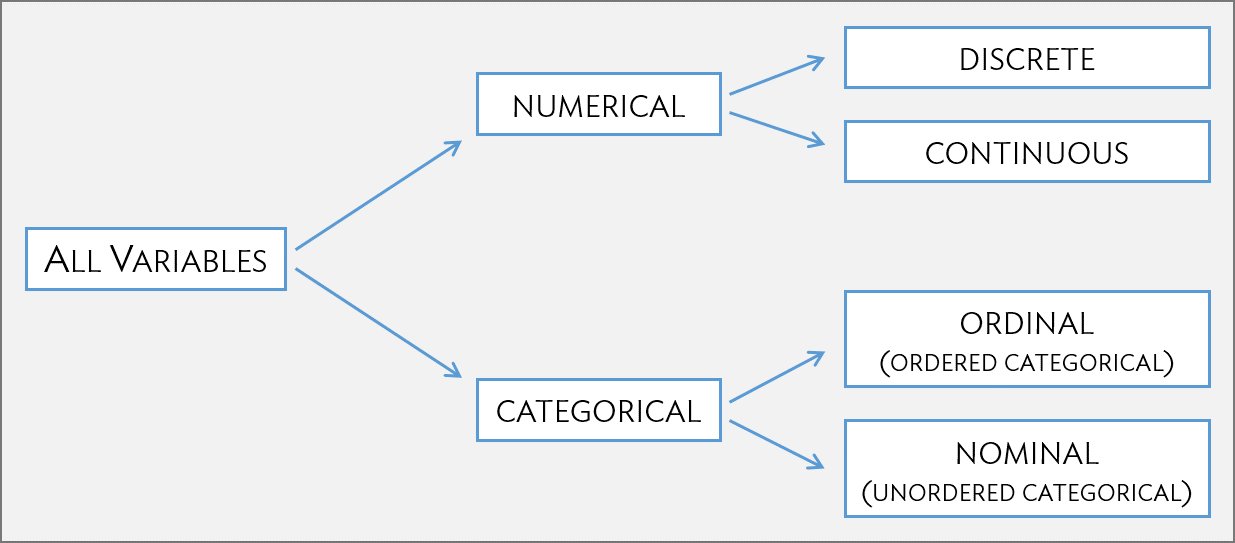
\includegraphics[width=0.70\textwidth]{ch_intro_to_data_oi_biostat/figures/variables/variableTypes.png}
\caption{Breakdown of variables into their respective types.}
\label{variableTypes}
\end{figure}

\begin{example}{Suppose at the beginning of a week a research assistant collected data on the first 20 individuals visiting one of the new walk-in clinics being offered by major commercial pharmacies.  In addition to other variables, the research assistant collected age (measured as less than 21, 21 - 65, and older than 65 years of age), sex, height, weight, and reason for the visit.  Classify each of the variables as continuous numerical, discrete numerical, or categorical.}
Height and weight are continuous numerical variables. Age as measured by the research assistant is ordered categorical. Sex and the reason for the visit are nominal categorical variables; sex has two categories, while reason for the visit will have many possible values. 
\end{example}


\begin{exercise} \index{!LEAP}
Characterize the variables \var{participant.ID}, \var{treatment.group}, and \var{overall.V60.outcome} from the LEAP study (discussed in Section~\ref{leapCaseStudy}). \footnote{These variables measure non-numerical quantities, and thus are categorical variables. The variables  \var{treatment.group} and \var{outcome.V60.overall} have two values or levels, while \var{participant.ID} has many possible values.}
\end{exercise}

\subsection{Relationships between variables}
\label{variableRelations}

Many studies are motivated by a researcher examining a possible relationship between two or more variables. Statistical relationships between two variables occur when they tend to vary in a related way. A \term{response variable} measures an outcome of interest, while an \term{explanatory variable} may be useful in predicting or understanding the response variable. There may be several possible explanatory variables for a single response variable in a given study.

Researchers were interested in using the \data{famuss} data to answer several questions, including: is ACTN3 genotype associated with variation in muscle function? The ACTN3 gene codes for a protein involved in muscle function. A common mutation (polymorphism) at residue 577 in the ACTN3 gene changes C to T; TT individuals are unable to produce any ACTN3 protein in their muscle. Thus, researchers hypothesized that ACTN3 genotype might influence muscle function in humans. The response variable in this study is \var{ndrm.ch}, the percent change in non-dominant arm strength, with strength gain being used as a way to measure muscle function. The explanatory variable of interest is \var{actn3.r557x}, ACTN3 genotype at residue 577.  

Both numerical and graphical ways to examine possible relationships between two variables will be covered later in the text.

\begin{example}{In the study conducted on Tibetan frogs, researchers collected measurements on egg clutches and female frogs at 11 study sites, located at differing altitudes. Identify the explanatory and response variables in the study.}
The explanatory variable examined in the study is \var{altitude}. The variables \var{egg.size}, \var{clutch.size}, \var{clutch.volume}, and \var{body.size} are response variables measuring the level of maternal investment. 
\end{example}	

\begin{exercise}
Refer to the variables from the \data{famuss} data set described in Table~\ref{famussVariables} to formulate two questions about the relationships between these variables that differ from the one addressed by the research team.\footnote{Two sample questions: (1)  Do participants appear respond differently to training according to race?  (2)  Do male participants appear to respond differently to training than females?}
\end{exercise}



\section{Data collection principles}
\label{dataCollectionPrinciples}

\index{sample|(}
\index{population|(}

The first step in research is to identify questions to investigate. A clearly articulated research question is essential for selecting subjects to be studied, identifying relevant variables, and determining how data should be measured. In order to obtain reliable data, it is also important to consider \textit{how} data are collected.

\subsection{Populations and samples}
\label{populationsAndSamples}

\begin{enumerate}
\setlength{\itemsep}{0mm}

\item What is the average mercury content in swordfish in the Atlantic Ocean?

\item If an infant seems predisposed to a peanut allergy, is it better to introduce or to avoid peanut products during the first 6 months of the infant's life?

\item What proportion of female college students experience sexual victimization?

\end{enumerate}

Each of these questions refers to a target \term{population}. In the first question, the target population is all swordfish in the Atlantic ocean, and each fish represents a case. Almost always, it is either too expensive or logistically impossible to collect data for every case in a population, so nearly all research is based on samples from populations. A \term{sample} represents a subset of the cases and is often a small fraction of the population. For instance, 60 swordfish (or some other number) in the population might be selected, and this sample data may be used (with some assumptions) to provide an estimate of the population average and answer the research question.



\subsection{Anecdotal evidence}
\label{anecdotalEvidence}

Anecdotal evidence is typically composed of unusual observations that are easily recalled based on their striking characteristics. Physicians are sometimes more likely to remember the characteristics of a single patient with an unusually good response to a drug as opposed to the many patients who did not respond.  The dangers of drawing general conclusions from anecdotal information are obvious; no single observation can be used to draw conclusions about a population. Often, the anecdotal case may not have been remembered correctly or may have been measured incorrectly. To learn about the characteristics of a population, it is necessary to examine a sample of many cases drawn randomly from the population.

While it is incorrect to generalize from individual observations, scientists know that unusual observations can sometimes be valuable.  E.C. Heyde was a general practitioner from Vancouver who noticed that a few of his elderly patients with aortic-valve stenosis (an abnormal narrowing) caused by an accumulation of calcium had suffered massive gastrointestinal bleeding, and in 1958, he published his observation in a letter. \footnote{Heyde EC. Gastrointestinal bleeding in aortic stenosis. N Engl J Med 1958;259:196.}.  Research into the problem led to the identification of the underlying cause of the association \footnote{Greenstein RJ, McElhinney AJ, Reuben D, Greenstein AJ. Co-lonic vascular ectasias and aortic stenosis: coincidence or causal relationship? Am J Surg 1986;151:347-51.}, now called Heyde's Syndrome.

An anecdotal observation can never be the basis for a conclusion, but it may well lead to the design of a more systematic study that could be definitive.  


\subsection{Sampling from a population}

Sampling from a population is a useful tool in population-based research in the health sciences.  When done carefully, it provides reliable information about the  characteristics of a large population without having to directly measure those characteristics for each member, often an impossible task.  The US Centers for Disease Control (US CDC) conducts many such surveys, including the Behavioral Risk Factors Surveillance System (BRFSS)\footnote{\url{ http://www.cdc.gov/brfss/}}.  The BRFSS conducts approximately 400,000 telephone interviews annually to ask U.S. residents questions regarding their health-related risk behaviors, chronic health conditions, and use of preventive services.  Data from a recent BRFSS are used in Chapter 4. The CDC conducts similar surveys for diabetes, health care access, and immunization. Likewise, the World Health Organization (WHO) conducts the World Health Survey in partnership  with approximately 70 countries to learn about the health of adult populations and the health systems in those countries.\footnote{\url{http://www.who.int/healthinfo/survey/en/}}  In 2000, the US Department of Justice released the \textit{The Sexual Victimization of College Women}, based on a survey conducted in 1996 of 4,446 undergraduate women.\footnote{\url{https://www.ncjrs.gov/pdffiles1/nij/182369.pdf}}

\begin{comment}
In September 2015, the American Association of Universities released a new study of the same issue\footnote{\url{https://www.aau.edu/uploadedFiles/AAU_Publications/AAU_Reports/Sexual_Assault_Campus_Survey/Report%20on%20the%20AAU%20Campus%20Climate%20Survey%20on%20Sexual%20Assault%20and%20Sexual%20Misconduct.pdf}}.

This url is causing latex compile problems.

\end{comment}


Sampling from a population is easier when the population is relatively small and members of the population are easy to identify and contact.  For instance, the quality improvement team at an integrated health care system, such as Kaiser Permanente or Harvard Pilgrim Health Care, might want to learn about the perception of care among members of the health plan.  Since health plans have contact information for each member, a selected subset can be contacted (with their consent) for participation in an interview or mailed survey.  More complex methods are required for other surveys, such as the study on sexual victimization of college women. 


One common pitfall in conducting a survey is to use a \term{convenience sample}\index{sample!convenience sample}, in which individuals who are easily accessible are more likely to be included in the sample. For instance, the quality improvement team in the healthcare plan might ask interviewers to approach plan members visiting an outpatient clinic during a particular week.  The sample would fail to enroll generally healthy members who typically do not use outpatient services or schedule routine physical examinations. Similarly, the Department of Justice could have only sampled women in colleges or universities in or near the District of Columbia or major state universities.  

\begin{figure}
	\centering
	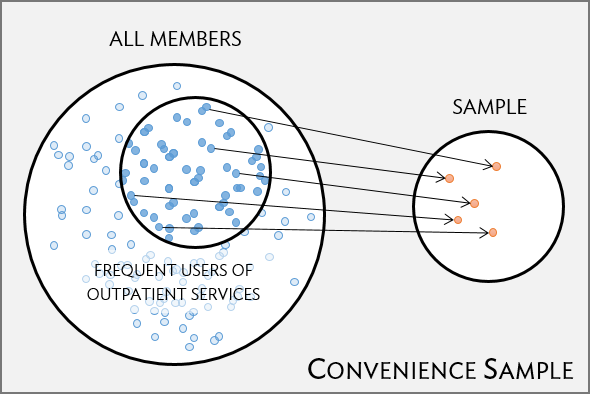
\includegraphics[width=0.70\textwidth]{ch_intro_to_data_oi_biostat/figures/sampleHealthPlan/sampleConvenienceHealthPlan.png}
	\caption{Instead of sampling from all members equally, approaching members visiting a clinic during a particular week would disproportionately select members who typically use outpatient services.}
	\label{sampleConvenienceHealthPlan}
\end{figure}

\index{sample!random sample|(}

The general principle of sampling is straightforward: a sample from a population is useful for learning about a population only when the sample matches, on average, the characteristics of the population. Random sampling is the best way to ensure that a sample reflects a population, because random samples are not subject to the conscious or unconscious bias of the team gathering the sample.  However, even a well-defined sampling strategy can lead to an unrepresentative sample if there are substantial barriers to subject participation, such as questions that assume participants are fluent in English or calls to potential participants that do not account for working hours or time-zone differences. 

The easiest random samples to analyze are those in which each member of a population has the same chance of being sampled. In a \term{simple random sample}, each member of the population is directly chosen at random for the sample, with probability the size of the sample divided by the size of the population. Simple random samples are essentially equivalent to how raffles are conducted. For example, if there are 5 prizes available and 100 people each have a single ticket, each person has a 5\% chance (5/100) of being called. In the health plan example, a subset of members might be chosen randomly from the plan membership roster for an interview. \textsl{OpenIntro}, third edition, Section 1.4.2 describes the four most commonly used sampling strategies. The link to the Department of Justice victimization survey describes in detail the design of the sampling plan for this study.

\begin{figure}[ht]
	\centering
	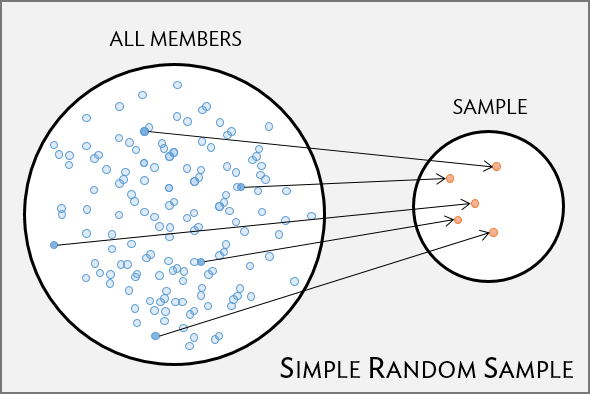
\includegraphics[width=0.70\textwidth]{ch_intro_to_data_oi_biostat/figures/sampleHealthPlan/sampleRandomHealthPlan.png}
	\caption{In this graphic, five members are randomly selected from the population to be interviewed.}
	\label{sampleRandomHealthPlan}
\end{figure}

The act of taking a simple random sample helps minimize bias, but bias can arise in other ways. Even when people are picked at random, caution must be exercised if the \term{non-response} rate \index{sample!non-response|textbf} is high. For instance, if only 30\% of the people randomly sampled for a survey respond, then it is unclear whether the results are truly \term{representative} of the entire population. Such \term{non-response bias} \index{sample!non-response bias|textbf} can skew results; it is important to minimize barriers that might discourage subject participation in order to collect reliable data.

\begin{figure}[h]
	\centering
	{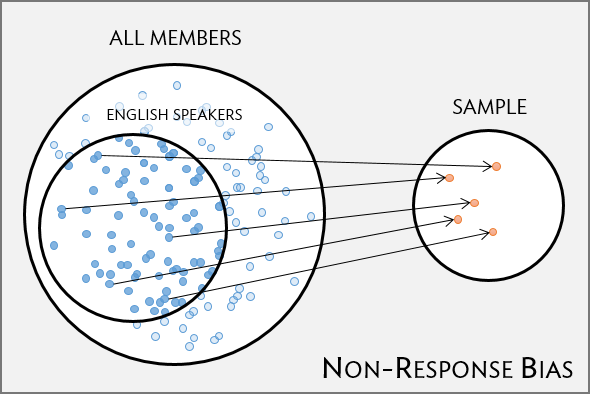
\includegraphics[width=0.70\textwidth]{ch_intro_to_data_oi_biostat/figures/sampleHealthPlan/sampleNonResponseHealthPlan.png}
	\caption{Due to the possibility of non-response, surveys studies may only reach a certain group within the population. For example, a survey written in English may only result in responses from health plan members fluent in English.}}
	\label{sampleNonResponseHealthPlan}
\end{figure}


\begin{exercise}
It is increasingly common for health care facilities to follow-up a patient visit with an email providing a link to a website where patients can rate their experience.  Typically, less than 50\% of patients visit the web site.  If half of those who respond indicate a negative experience, do you think that this implies that at least 25\% of patient visits are unsatisfactory?	\footnote{Answers will vary. If our experience is any guide, dissatisfied people to respond more frequently to these informal surveys than satisfied patients.}
\end{exercise}

\index{sample!random sample|)}
\index{population|)}
\index{sample|)}

\subsection{Introducing experiments and observational studies}

Experiments and observational studies are the two primary types of study designs used to collect data.

When researchers want to investigate the possibility of a causal connection, they conduct an \term{experiment}. The LEAP study team hypothesized that early exposure to peanut products would reduce the likelihood of an allergy to peanuts by age 5. To find evidence for a causal connection between the explanatory and response variables, researchers randomly assign a sample of individuals to one of two groups.  One group, called the experimental group, receives the intervention (peanut products in LEAP). In the other group, the control group, participants typically receive either a standard approach (avoiding peanut products in LEAP) or may receive either a \term{placebo}, an inert substance with the appearance of the experimental intervention.  Placebos are used to prevent participants from knowing their assigned treatment, but they are not feasible in all studies.

Scientists conduct an \term{observational study} when they collect data in a way that does not interfere with how the data arise. For instance, to study why certain diseases develop, researchers may collect information through conducting surveys, reviewing medical or company records, or following a \term{cohort} of many similar individuals. In each of these situations, researchers merely observe the data that arise. Observational studies can provide evidence of an association between variables, but they cannot by themselves show a causal connection. In general, causation can only be inferred from a randomized experiment.

\subsection[Experiments]{Experiments}
\label{experiments}

Studies in which researchers assign treatments to cases are called \termsub{experiments}{experiment}. Randomized experiments, called randomized clinical trials in medicine and the social and behavioral sciences, are an essential tool in research and public policy.  For all but a few exceptional settings,  The US Food and Drug Administration requires that two independently conducted randomized trials confirm that a new drug is safe and effective before it can be marketed,  and the European Medicines Agency has a similar policy.  

Randomized experiments are generally built on three principles.

\index{data!LEAP|(}

\begin{description}

	\item[Control.] Researchers select participants for the study in a way reduces unnecessary variability, doing their best to \term{control} for variables that might make the results difficult to interpret. For instance, participants are selected from individuals who have aspects of a disease or condition that suggests they may benefit from the intervention being studied. All infants enrolled in the LEAP study were required to be between 4 and 11 months of age, with severe eczema and/or allergies to eggs.

	\item[Randomization.] Researchers randomize patients into treatment groups to account for variables that cannot be controlled. For example, some infants may have been more susceptible to peanut allergies because of an unmeasured genetic condition. Randomly assigning patients to the treatment or control group helps even out such differences between the two groups. In situations where researchers suspect that variables other than the treatment may influence the response, they may first group individuals into \term{blocks} and then, within each block, randomize cases to treatment groups; this technique is referred to as \term{blocking} or \term{stratification}.  In the LEAP study, infants were stratified into two cohorts based on whether or not the child developed a red, swollen mark (a wheal) after a skin test at the time of enrollment. The main analysis of the study analyzed data collected for infants without a wheal after the skin test. Figure~\ref{leapBlocking} illustrates the blocking scheme used in the study. General methods for analyzing blocked data are relatively complicated and will not be covered in this book.

	\item[Replication.] The more cases researchers observe, the more accurately they can estimate the effect of the explanatory variable on the response. In a single study, \term{replication} is accomplished by collecting a sufficiently large sample. The LEAP study randomized a total of 640 infants; 542 infants were in the block without the wheal response. 

\end{description}

It is important to incorporate the three experimental design principles into any study; this book describes applicable methods for analyzing data from such experiments. Blocking is a slightly more advanced technique, and statistical methods in this book may be extended to analyze data collected using blocking.

	\begin{figure}
		\centering
		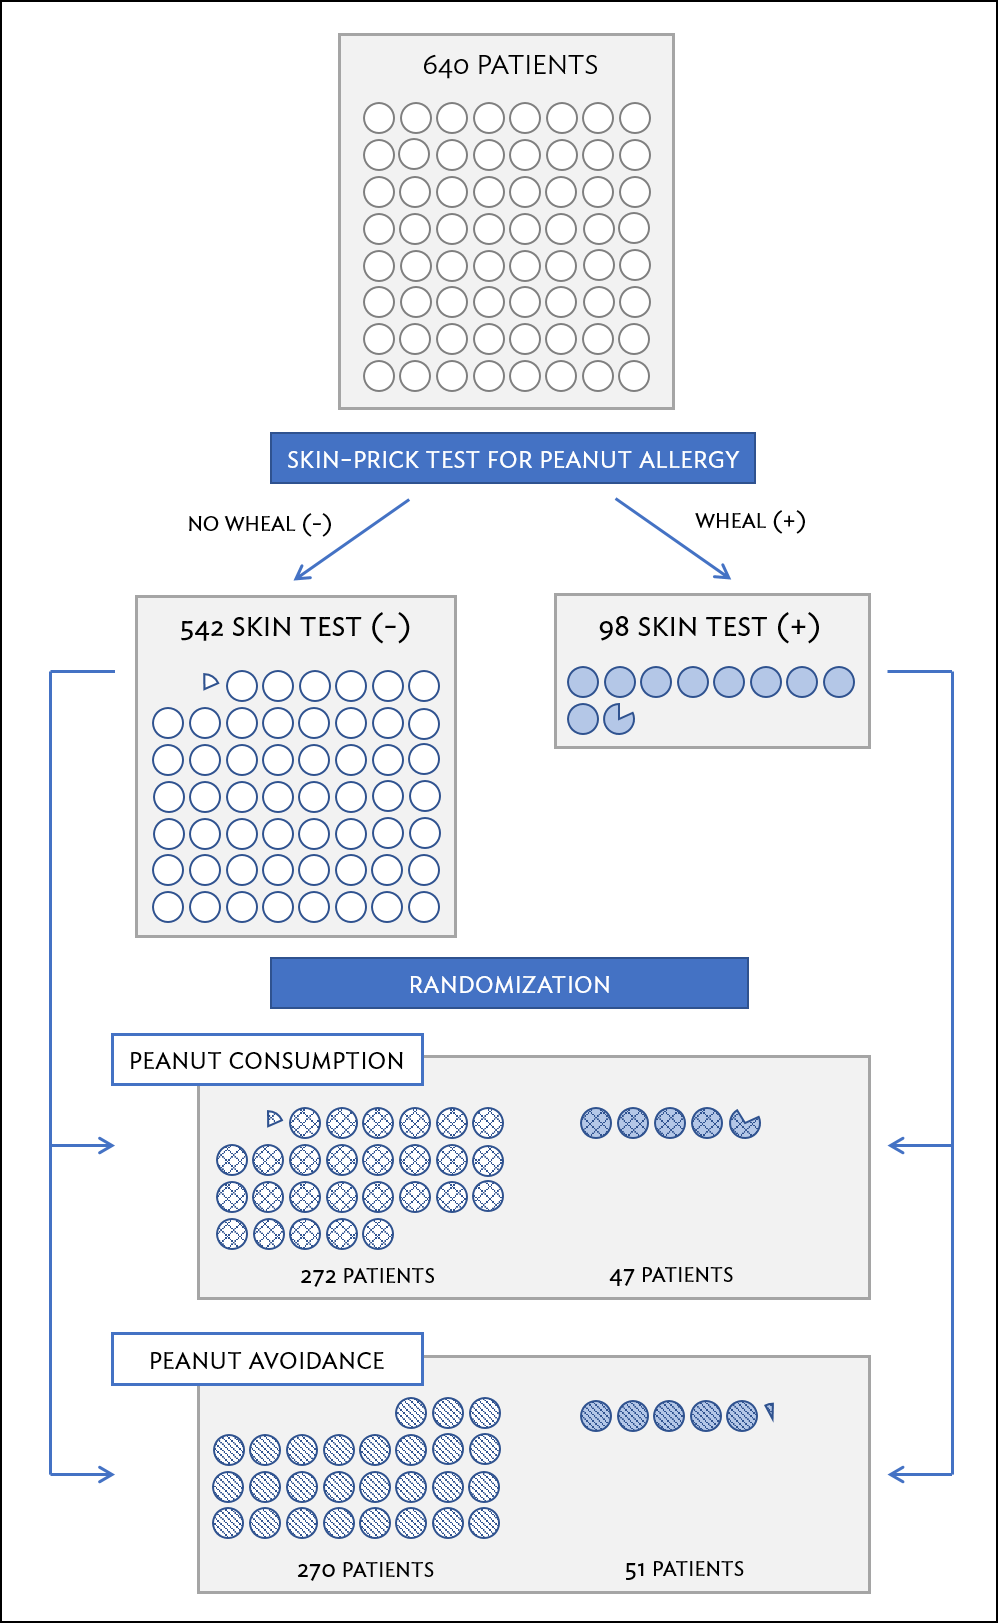
\includegraphics[width=0.78\textwidth]{ch_intro_to_data_oi_biostat/figures/leapBlocking/leapBlocking.png}
		\caption{A simplified schematic of the blocking scheme used in the LEAP study, depicting 54 patients that underwent randomization. Patients are first divided into groups based on response to the initial skin test, then each block is evenly separated into the treatment groups using randomization. This strategy ensures an even representation of patients in each treatment group from both the skin test positive and skin test negative groups.}
		\label{leapBlocking}
	\end{figure}

\index{data!LEAP|)}

\subsection{Reducing bias in human experiments}
\label{biasInHumanExperiments}

Randomized experiments are the gold standard for data collection, but they do not automatically ensure an unbiased perspective in all cases. Human studies are perfect examples where bias can arise unintentionally. 

In 1980, researchers reported the results of a study assessing the efficacy of a new drug used to treat heart attack patients.\footnote{Anturane Reinfarction Trial Research Group. 1980. Sulfinpyrazone in the prevention of sudden death after myocardial infarction. New England Journal of Medicine 302(5):250-256.} Researchers wanted to know whether the drug reduced deaths in patients; in order to draw causal conclusions about the effect of the drug, they designed a randomized experiment in which study volunteers were randomly assigned to one of two study groups.\footnote{Human subjects are often called \term{volunteers}, or \term{study participants}.} The \term{treatment group} received the drug; the \term{control group} did not receive any drug treatment.

Typically, researchers do not want patients to know which group they are in. The emotional response of a patient who knows they are either receiving or not receiving a potentially helpful new drug may cause different behavior between the two groups. In order to eliminate this source of bias from the study, researchers conduct a \term{blinded} study in which patients are kept uninformed about their treatment. Patients in the control group, instead of being given a drug, are given an inert substance called a \term{placebo}. An effective placebo is the key to making a study truly blind. A placebo may often result in a slight but real improvement in patients; this effect is referred to as the \term{placebo~effect}.\footnote{Kaptchuk, TJ and Miller, FG. 2015.Placebo effects in medicine, New England Journal of Medicine, 373(1):8-9.}

The patients are not the only ones who should be blinded: doctors and researchers can accidentally bias a study. For example, out of concern for potential side effects of a new drug, a doctor might inadvertently give a patient in the treatment group more attention and care than they would to a patient known to be taking a placebo. To guard against this bias, which has also been found to have a measurable effect, many modern studies use a \term{double-blind} design in which doctors who interact with patients are, just like the patients, unaware of who is or is not receiving the experimental treatment.\footnote{There are always some researchers involved in the study who do know which patients are receiving which treatment. However, they do not directly interact with patients and do not tell the blinded health care professionals who is receiving which treatment.}

\begin{exercise}
	Look back to the study in Section~\ref{leapCaseStudy} in which researchers were testing whether peanut product consumption was effective at reducing the likelihood of peanut allergies in children at-risk for these allergies. Is this an experiment? Was the study blinded? Was it double-blinded? \footnote{The researchers assigned the patients into their treatment groups, so this study was an experiment. However, the patients (and their parents) could distinguish which treatment they received, so this study was not blind. The study could not be double-blind since it was not blind.}
\end{exercise}

\subsection{Observational studies}

While experiments require researchers to assign the primary explanatory variable (i.e., the intervention) to each subject, in observational studies researchers simply observe selected potential explanatory and response variables. Participants who differ in important explanatory variables may also differ in other ways that influence response.  Observational studies of obesity have shown that obese individuals tend to die sooner that individuals with normal weight, but obese individuals usually have other health behaviors that influence life expectancy, such as reduced exercise. Making causal conclusions based on experiments is often reasonable; however, making the same causal conclusions solely based on observational data should be avoided. 

Suppose an observational study tracked sunscreen use and skin cancer, finding that the more sunscreen a person uses, the more likely they are to have skin cancer. However, this does not mean that sunscreen \emph{causes} skin cancer. One important piece of missing information is sun exposure -- if someone is out in the sun all day, they are both more likely to use sunscreen and to get skin cancer. Sun exposure is a  \term{confounding variable}: a variable correlated with both the explanatory and response variables.\footnote{Also called a \term{lurking variable}, \term{confounding factor}, or a \term{confounder}.} There is no guarantee that all confounding variables can be examined or measured; as a result, it is difficult to justify making causal conclusions from observational studies. 
% Some studies:
% http://www.sciencedirect.com/science/article/pii/S0140673698121682
% http://archderm.ama-assn.org/cgi/content/abstract/122/5/537
% Study with a similar scenario to that described here:
% http://onlinelibrary.wiley.com/doi/10.1002/ijc.22745/full

\begin{center}
	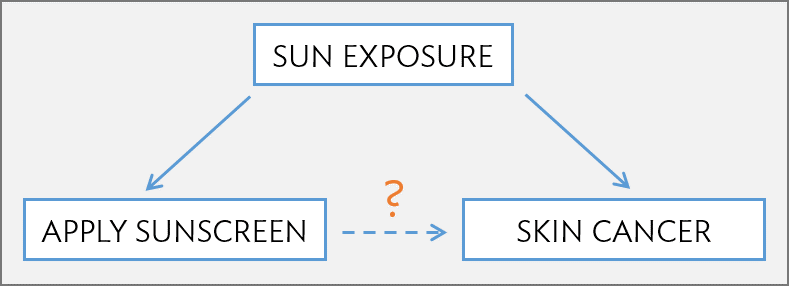
\includegraphics[height=1.25in]{ch_intro_to_data_oi_biostat/figures/variables/confoundingVariable.png}
\end{center}

Observational studies can reveal interesting patterns or important associations useful for designing follow-up experiments. Several observational studies based on dietary data from different countries showed a strong association between dietary fat and breast cancer in women.  These observations were the basis for The Women's Health Initiative (WHI), a large randomized trial sponsored by the US NIH.  In the WHI, women were randomized to standard vs low fat diets, and the previously observed association was not confirmed.  \textit{If we keep this example, we need references.}

Observational studies can be either prospective or retrospective. A \term{prospective study} identifies participants and collects information at scheduled times or as events unfold. For instance, medical researchers may identify and follow a group of similar individuals over many years to assess the possible influences of behavior on cancer risk. One example of such a study is The Nurses' Health Study, started in 1976 and expanded in 1989.\footnote{\texttt{\oiRedirect{textbook-channing_nurse_study}{www.channing.harvard.edu/nhs}}} This prospective study recruits registered nurses and then collects data using questionnaires. \termsub{Retrospective studies}{retrospective studies} collect data after events have taken place, e.g. researchers may review past events in medical records. Some datasets may contain both prospectively- and retrospectively-collected variables. The Cancer Care Outcomes Research and Surveillance Consortium (CanCORS)\footnote{Ayanian, John Z., et al. "Understanding cancer treatment and outcomes: the cancer care outcomes research and surveillance consortium." Journal of Clinical Oncology 22.15 (2004): 2992-2996} enrolled participants with lung or colorectal cancer, collected information about diagnosis, treatment and previous health behavior, but also maintained contact with participants to gather data about long term outcomes.  


\subsection{Four sampling methods (special topic)}

\textit{To be inserted in a subsequent draft.}

\begin{comment}

\label{fourSamplingMethods}
\label{threeSamplingMethods}

Almost all statistical methods are based on the notion of implied randomness. If observational data are not collected in a random framework from a population, these statistical methods -- the estimates and errors associated with the estimates -- are not reliable. Here we consider four random sampling techniques: simple, stratified, cluster, and multistage sampling. Figures~\ref{simple_stratified} and~\ref{cluster_multistage} provide graphical representations of these techniques.

\begin{figure}
\centering
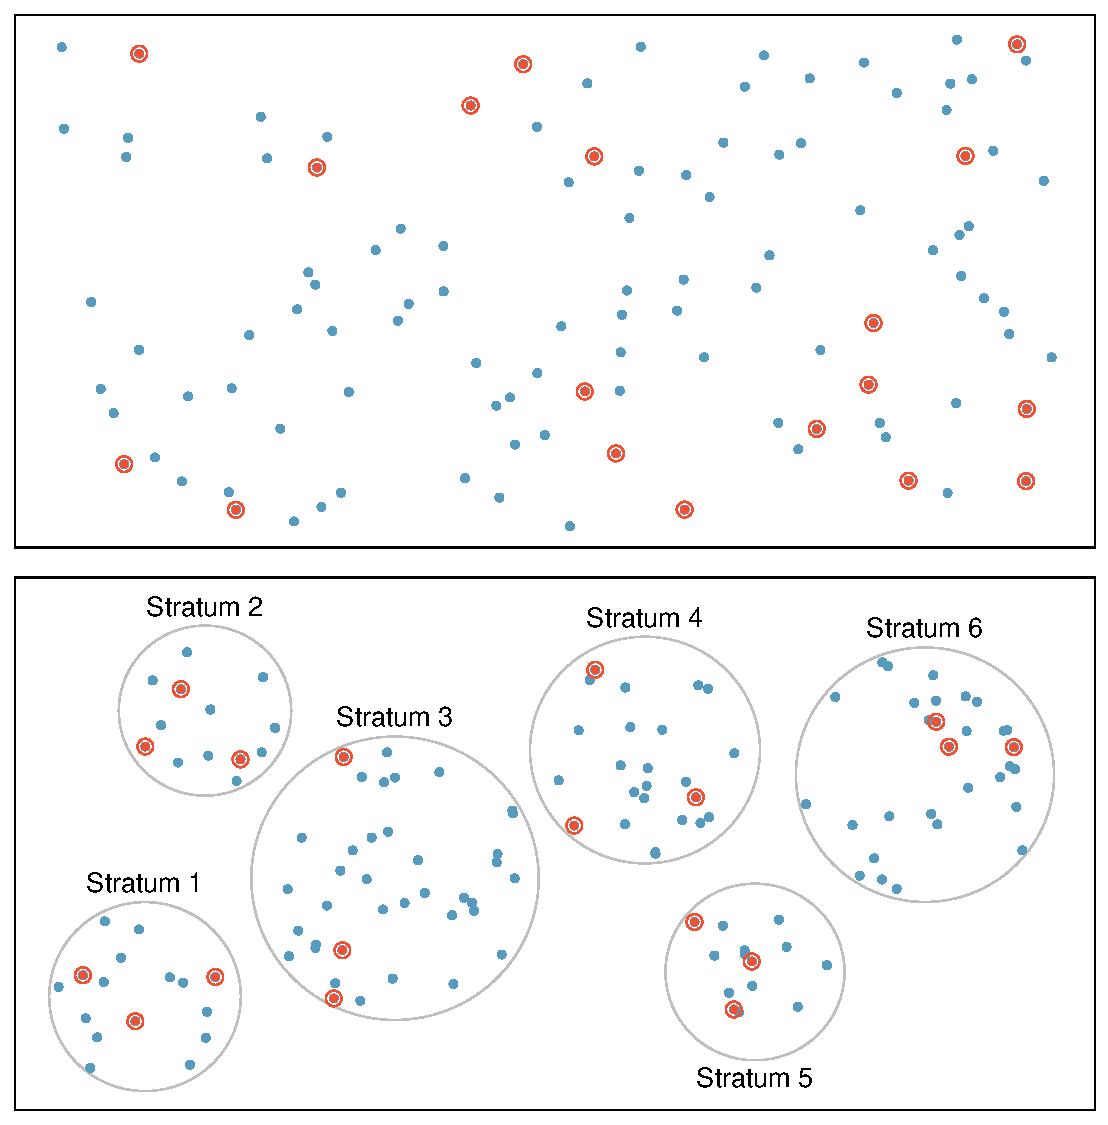
\includegraphics[width=\textwidth]{ch_intro_to_data_oi_biostat/figures/samplingMethodsFigure/simple_stratified}
\caption{Examples of simple random\index{sample!simple random sampling} and stratified sampling\index{sample!stratified sampling}. In the top panel, simple random sampling was used to randomly select the 18 cases. In the bottom panel, stratified sampling was used: cases were grouped into strata, then simple random sampling was employed within \mbox{each stratum}.}
\label{simple_stratified}
\end{figure}

\termsub{Simple random sampling}{sample!simple random sampling} is probably the most intuitive form of random sampling. Consider the salaries of Major League Baseball (MLB) players, where each player is a member of one of the league's 30 teams. To take a simple random sample of 120 baseball players and their salaries from the 2010 season, we could write the names of that season's 828 players onto slips of paper, drop the slips into a bucket, shake the bucket around until we are sure the names are all mixed up, then draw out slips until we have the sample of 120 players. In general, a sample is referred to as ``simple random'' if each case in the population has an equal chance of being included in the final sample \emph{and} knowing that a case is included in a sample does not provide useful information about which other cases are included.

\termsub{Stratified sampling}{sample!stratified sampling} is a divide-and-conquer sampling strategy. The population is divided into groups called \term{strata}\index{sample!strata|textbf}. The strata are chosen so that similar cases are grouped together, then a second sampling method, usually simple random sampling, is employed within each stratum. In the baseball salary example, the teams could represent the strata, since some teams have a lot more money (up to 4~times as much!). Then we might randomly sample 4 players from each team for a total of 120 players.

Stratified sampling is especially useful when the cases in each stratum are very similar with respect to the outcome of interest. The downside is that analyzing data from a stratified sample is a more complex task than analyzing data from a simple random sample. The analysis methods introduced in this book would need to be extended to analyze data collected using stratified sampling.

\begin{example}{Why would it be good for cases within each stratum to be very similar?}
We might get a more stable estimate for the subpopulation in a stratum if the cases are very similar. These improved estimates for each subpopulation will help us build a reliable estimate for the full population.
\end{example}

In a \termsub{cluster sample}{sample!cluster sample}, we break up the population into many groups, called \termsub{clusters}{sample!cluster}. Then we sample a fixed number of clusters and include all observations from each of those clusters in the sample. A \termsub{multistage sample}{sample!multistage sample} is like a cluster sample, but rather than keeping all observations in each cluster, we collect a random sample within each selected cluster. %Multistage sampling is similar to stratified sampling in its process, except that stratified sampling requires observations be sampled from \emph{every} stratum.

\begin{figure}
\centering
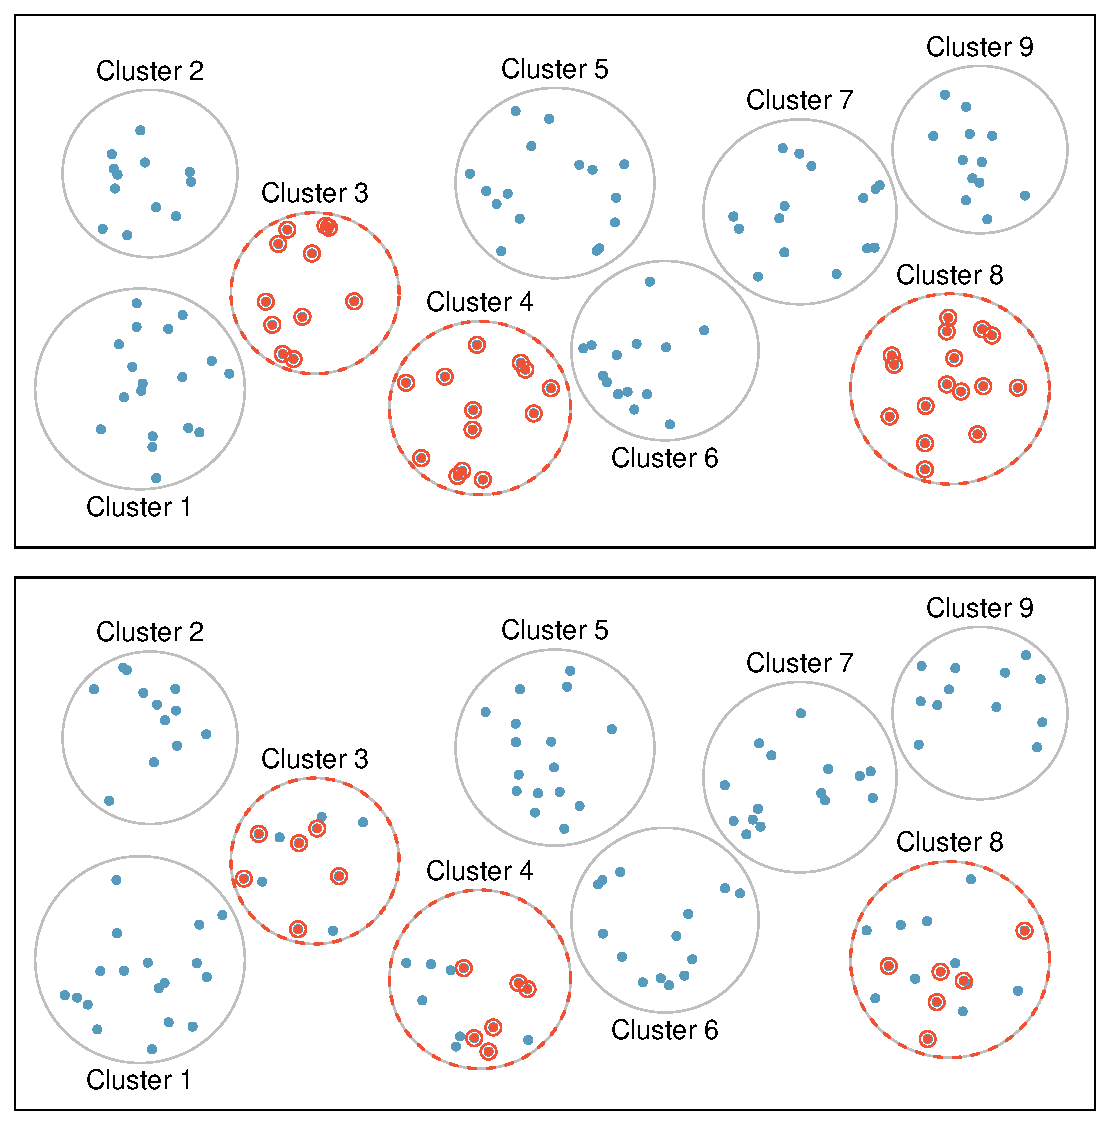
\includegraphics[width=\textwidth]{ch_intro_to_data_oi_biostat/figures/samplingMethodsFigure/cluster_multistage}
\caption{Examples of cluster\index{sample!cluster sampling} and multistage sampling\index{sample!multistage sampling}. In the top panel, cluster sampling was used. Here, data were binned into nine clusters, three of these clusters were sampled, and all observations within these three cluster were included in the sample. In the bottom panel, multistage sampling was used.
It differs from cluster sampling in that of the clusters selected, we randomly select a subset of each cluster to be included in the sample.}
\label{cluster_multistage}
\end{figure}

Sometimes cluster or multistage sampling can be more economical than the alternative sampling techniques. Also, unlike stratified sampling, these approaches are most helpful when there is a lot of case-to-case variability within a cluster but the clusters themselves don't look very different from one another. For example, if neighborhoods represented clusters, then cluster or multistage sampling work best when the neighborhoods are very diverse. A downside of these methods is that more advanced analysis techniques are typically required, though the methods in this book can be extended to handle such data.

\begin{example}{Suppose we are interested in estimating the malaria rate in a densely tropical portion of rural Indonesia. We learn that there are 30 villages in that part of the Indonesian jungle, each more or less similar to the next. Our goal is to test 150 individuals for malaria. What sampling method should be employed?}
A simple random sample would likely draw individuals from all 30 villages, which could make data collection extremely expensive. Stratified sampling would be a challenge since it is unclear how we would build strata of similar individuals. However, cluster sampling or multistage sampling seem like very good ideas. If we decided to use multistage sampling, we might randomly select half of the villages, then randomly select 10 people from each. This would probably reduce our data collection costs substantially in comparison to a simple random sample, and this approach would still give us reliable information.
\end{example}

\end{comment}

\section[Examining numerical data]{Examining numerical data}
\label{numericalData}

\index{data!frog|(}

This section introduces techniques for exploring and summarizing numerical variables, using the \data{frog} data from Section~\ref{dataBasics}.

\subsection{Measures of center: mean and median}
\label{measuresOfCenter}

The \term{mean}, sometimes called the \indexthis{average}{mean!average}, is a common way to measure the center of a \term{distribution} of data. To find the average clutch volume for the observed egg clutches, we add up all the clutch volumes and divide by the total number of clutches. For computational convenience, the volumes are rounded to the first~decimal.
\begin{eqnarray}
\overline{x} = \frac{177.8 + 257.0 + \cdots + 933.3}{431} = 882.5\ \textrm{mm}^{3}
\label{sampleMeanEquation}
\end{eqnarray}
The sample mean is often labeled $\overline{x}$\marginpar[\raggedright$\overline{x}$\\\footnotesize sample\\ mean]{\raggedright$\overline{x}$\\\footnotesize sample\\ mean}. The letter $x$ is being used as a generic placeholder for the variable of interest, \var{clutch.volume}, and the bar over the $x$ communicates that the average volume of the 431 clutches is $882.5\textrm{mm}^{3}$. 


\begin{termBox}{\tBoxTitle{Mean}%
		The sample mean of a numerical variable is the sum of all observations divided by the number of observations:
		\begin{eqnarray}
		\overline{x} = \frac{x_1+x_2+\cdots+x_n}{n}
		\label{meanEquation}
		\end{eqnarray}
		where $x_1, x_2, \dots, x_n$ represent the $n$ observed values.}
\end{termBox}

\begin{comment}
\marginpar[\raggedright\vspace{-8mm}
$n$\\\footnotesize sample size]{\raggedright\vspace{-8mm}
$n$\\\footnotesize sample size}\vspace{-2mm}
\end{comment}

The \term{median} is another measure of center; it is the middle number in a distribution after the values have been ordered from smallest to largest. If the distribution contains an even number of observations, the median is the average of the middle two observations. There are 431 clutches in the dataset, so the median is the clutch volume of the $216^{th}$ observation in the sorted values of \var{clutch.volume}: $831.8\ \textrm{mm}^{3}$.




\subsection{Measures of spread: standard deviation and interquartile range}
\label{measuresOfSpread}


The standard deviation measures (approximately) the distance between a typical observation and the mean. The distance of an observation from its mean its \term{deviation}. Below are the deviations for the $1^{st}$, $2^{nd}$, $3^{rd}$, and $431^{th}$ observations in the \var{clutch.volume} variable. For computational convenience, clutch volume is rounded to the first decimal.

\begin{align*}
x_1-\overline{x} &= 177.8 - 882.5 = -704.7 \hspace{5mm}\text{ } \\
x_2-\overline{x} &= 257.0 - 882.5 = -625.5 \\
x_3-\overline{x} &= 151.4 - 882.5 = -731.1 \\
&\ \vdots \\
x_{431}-\overline{x} &= 933.2 - 882.5 = 50.7
\end{align*}
% library(openintro); d <- frog.altitude$clutch.volume; round(mean(d),1); d[c(1,2,3,431)]; d[c(1,2,3,431)] - round(mean(d),1); (d[c(1,2,3,431)] - round(mean(d)))^2; sum((d - round(mean(d)))^2)/49; sqrt(sum((d - round(mean(d)))^2)/49); var(d); sd(d)

The sample \term{variance}\label{varianceFirstDiscussed}, is the average of the square of these deviations, and is  denoted by $s^2$\marginpar[\raggedright$s^2$\\\footnotesize sample variance]{\raggedright$s^2$\\\footnotesize sample variance}:
\begin{align*}
s^2 &= \frac{(-704.7)^2 + (-625.5)^2 + (-731.1)^2 + \cdots + (50.7)^2}{431-1} \\
&= \frac{496,602.09 + 391,250.25 + 534,507.21 + \cdots + 2570.49}{430} \\
&= 143,680.9
\end{align*}
The denominator is $n-1$ rather than $n$ when computing the variance; this mathematical nuance comes from statistical theory and the reason for doing so is not covered in this text.

The \term{standard deviation} is the square root of the variance:
$$s=\sqrt{143,680.9} = 379.05$$
\marginpar[\raggedright\vspace{-10mm}

$s$\\\footnotesize sample standard deviation]{\raggedright\vspace{-10mm}
$s$\\\footnotesize sample standard deviation
}\index{s@$s$} The standard deviation of clutch volume for the egg clutches observed is about $380\ \textrm{mm}^{3}$. 


\begin{comment}
\begin{figure}
\centering
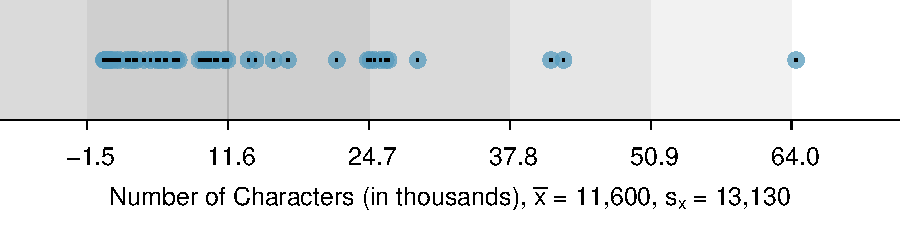
\includegraphics[width=\mycaptionwidth]{ch_intro_to_data_oi_biostat/figures/sdAsRuleForEmailNumChar/sdAsRuleForEmailNumChar}
\caption{In the \var{num\_\hspace{0.3mm}char} data, 41 of the 50 emails (82\%) are within 1~standard deviation of the mean, and 47 of the 50 emails (94\%) are within 2 standard deviations. Usually about 70\% of the data are within 1 standard deviation of the mean and 95\% are within 2 standard deviations, though this rule of thumb is less accurate for skewed data, as shown in this example.}
\label{sdAsRuleForEmailNumChar}
\end{figure}
\end{comment}

Formulas and methods used to compute the variance and standard deviation for a population are similar to those used for a sample.\footnote{The only difference is that the population variance has a division by $n$ instead of $n-1$.} However, like the mean, the population values have special symbols: $\sigma_{}^2$\marginpar[\raggedright$\sigma_{}^2$\\\footnotesize population variance\\ \hspace{2mm}]{\raggedright$\sigma_{}^2$\\\footnotesize population variance\\ \hspace{2mm}} for the variance and $\sigma$\marginpar[\raggedright$\sigma$\\\footnotesize population standard deviation\\ \hspace{2mm}]{\raggedright$\sigma$\\\footnotesize population standard deviation\\ \hspace{2mm}} for the standard deviation. The symbol $\sigma$ \index{Greek!sigma@sigma ($\sigma$)} is the Greek letter \emph{sigma}.


\begin{comment}
\begin{tipBox}{\tipBoxTitle{standard deviation describes variability}
		Focus on the conceptual meaning of the standard deviation as a descriptor of variability rather than the formulas. Usually 70\% of the data will be within one standard deviation of the mean and about 95\% will be within two standard deviations. However, as seen in Figures~\ref{sdAsRuleForEmailNumChar} and~\ref{severalDiffDistWithSdOf1}, these percentages are not strict rules.}
\end{tipBox}
\end{comment}

\begin{termBox}{\tBoxTitle{Standard Deviation}
		The sample standard deviation of a numerical variable is computed as the square root of the variance, which is the sum of squared deviations divided by the number of observations minus 1.
		\begin{eqnarray}
		s = \sqrt{\frac{({x_1 - \overline{x})}^{2}+({x_2 - \overline{x})}^{2}+\cdots+({x_n - \overline{x})}^{2}}{n-1}}
		\label{SDEquation}
		\end{eqnarray}
		where $x_1, x_2, \dots, x_n$ represent the $n$ observed values.}
\end{termBox}

Variability can also be measured using the \term{interquartile range} (IQR).  To calculate the IQR, find the \term{first quartile} \index{quartile!first quartile ($Q_1$)} (the $25^{th}$ \hiddenterm{percentile}, i.e. 25\% of the data fall below this value) and the \term{third quartile} \index{quartile!third quartile ($Q_3$)} (the $75^{th}$ percentile). These are often labeled $Q_1$ and $Q_3$, respectively. The IQR is the difference: $Q_3 - Q_1$.

The IQR for \var{clutch.volume} is $1096.0 - 609.6 = 486.4\ \textrm{mm}^{3}$.  The middle $50\%$ of the values for \var{clutch.volume} lie between $609.6\ \textrm{mm}^{3}$ and $1096.0\ \textrm{mm}^{3}$.

\subsection{Robust statistics}

In the \data{frog} data, there are four observed clutch volumes larger than 2,000 $\textrm{mm}^{3}$ (2138.0, 2630.3, 2454.7, 2511.9). These values can be clearly identified by plotting the data as points on a single axis, as shown in Figure~\ref{frogClutchVolDotPlot}; this graphical display is a \term{dot plot}. How do these extreme values affect the summary statistics for the clutch volume variable in the \data{frog} data?

\begin{figure}[ht]
	\centering
	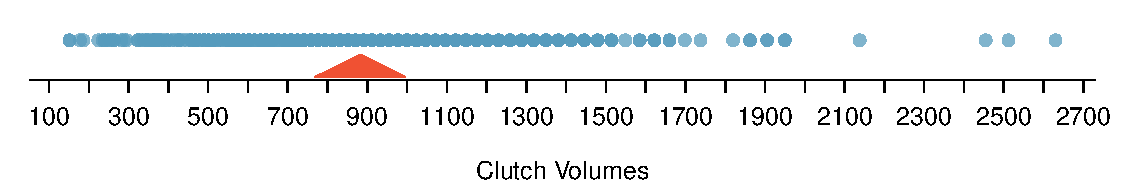
\includegraphics[width=\textwidth]{ch_intro_to_data_oi_biostat/figures/frogClutchVolDotPlot/frogClutchVolDotPlot}
	\caption{Dot plot of the clutch volume variable in the \data{frog} data.}
	\label{frogClutchVolDotPlot}
\end{figure}

The sample statistics are computed under each of two scenarios in Table~\ref{frogRobustOrNotTable}, one with and one without the four largest observations. The median and IQR are referred to as \term{robust estimates} because extreme observations have little effect on their values. For these data, the median does not change, while the IQR differs by only about 6 $\textrm{mm}^{3}$. In contrast, the mean and standard deviation are much more affected, particularly the standard deviation; since standard deviation depends on the squared distances from the mean, its change in the presence of large observations is more noticeable. Typically, extreme observations have a greater effect on the standard deviation than on the mean.

\begin{table}[ht]
	\centering
	\begin{tabular}{l c cc c cc}
		\hline
		& \hspace{0mm} & \multicolumn{2}{c}{\bf robust} & \hspace{2mm} & \multicolumn{2}{c}{\bf not robust} \\
		scenario && median & IQR && $\overline{x}$ & $s$ \\ 
		\hline
		original \var{frog} data 	&& 831.8 & 486.9 && 882.5 & 379.1 \\
		% library(openintro); data(frog.altitude); d <- frog.altitude$clutch.volume; median(d); IQR(d); mean(d); sd(d)
		drop four largest observations && 831.8 & 493.92 && 867.9 & 349.2 \\
		% library(openintro); data(frog.altitude); d <- frog.altitude$clutch.volume; a <- d<= 2000; median(d[a]); IQR(d[a]); mean(d[a]); sd(d[a])
		\hline
	\end{tabular}
	\caption{A comparison of how the median, IQR, mean ($\overline{x}$), and standard deviation ($s$) change when extreme observations are present.}
	\label{frogRobustOrNotTable}
\end{table}

If the dots in figure~\ref{frogClutchVolDotPlot} are thought of as small balls of equal weight distributed along a rod, the red triangle at the mean of the data is the balance point for the rod. This leads to the interpretation of the mean as the balance point or center of mass of a distribution. This physical analogy helps explain why large observations can influence the value of the mean.  The balance point has to be moved to the right, for instance, if a point is placed at the extreme right end of the rod.


\subsection{Visualizing distributions of data: histograms and boxplots}
\label{histogramsBoxplots}

Graphs of distributions, such as histograms and boxplots, show important features that are not evident in numerical summaries.  These features may include asymmetry, outliers, peaks or clumps in a distribution where some values are more likely than others, or values that are impossible and have been measured in error.

Dot plots show the exact value of each observation; while this is useful for small datasets, dot plots are not ideal for larger samples. Instead, observations can be grouped into bins and plotted as bars to form a \term{histogram}. Table~\ref{frogBinnedClutchVolTable} shows the number of clutches with volume between 0 and 200 $\textrm{mm}^{3}$, 200 and 400 $\textrm{mm}^{3}$, etc. up until 2,600 and 2,800 $\textrm{mm}^{3}$. These binned counts are plotted in Figure~\ref{frogHist}.

\begin{table}[ht]
	\centering\small
	\begin{tabular}{l ccc ccc ccc c}
		\hline
		\raisebox{-1.5ex}[0pt]{Clutch volumes} & \\
		& \raisebox{1.5ex}[0pt]{0-200} & \raisebox{1.5ex}[0pt]{200-400} & \raisebox{1.5ex}[0pt]{400-600} & \raisebox{1.5ex}[0pt]{600-800} & \raisebox{1.5ex}[0pt]{$\cdots$} & \raisebox{1.5ex}[0pt]{2400-2600} & \raisebox{1.5ex}[0pt]{2600-2800} \\
		\hline
		\raisebox{-.25ex}[0pt]{Count} & \raisebox{-.25ex}[0pt]{4} & \raisebox{-.25ex}[0pt]{29} & \raisebox{-.25ex}[0pt]{69} & \raisebox{-.25ex}[0pt]{99} & \raisebox{-.25ex}[0pt]{$\cdots$} & \raisebox{-.25ex}[0pt]{2} & \raisebox{-.25ex}[0pt]{1} \\
		\hline
	\end{tabular}
	\caption{The counts for the binned \var{clutch.volume} data.}
	\label{frogBinnedClutchVolTable}
\end{table}
% hist(frog.altitude$clutch.volume, breaks = 14, plot = FALSE)

\begin{figure}[ht]
	\centering
	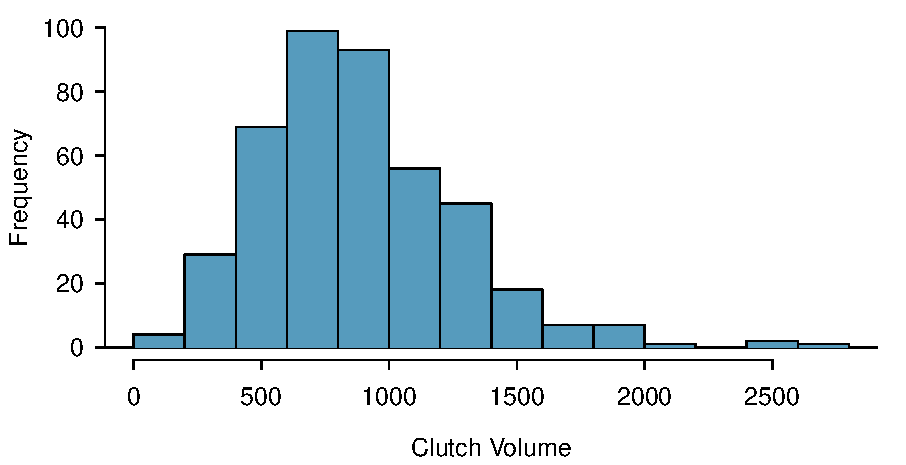
\includegraphics[width=0.82\textwidth]{ch_intro_to_data_oi_biostat/figures/frogHist/frogHist}
	\caption{A histogram of \var{clutch.volume}.}
	\label{frogHist}
\end{figure}

Histograms provide a view of the \term{data density}. Higher bars indicate more frequent observations, while lower bars represent relatively rare observations. For instance, there are many more egg clutches with volumes smaller than 1,500 $\textrm{mm}^{3}$ than clutches with larger volumes. The bars make it easy to see how the density of the data changes with clutch volume.

Histograms are especially convenient for describing the shape of the data distribution\label{shapeFirstDiscussed}. Figure~\ref{frogHist} shows that most clutches have a relatively small volume, while fewer clutches are very large. When data trail off to the right, with a long right \hiddenterm{tail}\index{skew!tail}, the data are said to be \termsub{right skewed}{skew!right skewed}.\footnote{Other ways to describe data that are skewed to the right: \termni{skewed to the right}, \termni{skewed to the high end}, or \termni{skewed to the positive end}.} Data with the reverse characteristic -- a long, thin tail to the left -- are said to be \termsub{left skewed}{skew!left skewed}. Right and left skewing are examples of asymmetry.  The term \term{symmetric} is used to describe data that show roughly equal trailing off in both directions.

The mean and standard deviation have a convenient interpretation in symmetric distributions.  Usually about 70\% of the data are within 1 standard deviation of the mean and 95\% are within 2 standard deviations, so simple numerical summaries provide approximate information on where the majority of the data are located.  This approximation, also known as the \term{empirical rule}, is not accurate for skewed distributions.  The empirical rule is discussed in more detail in Chapter 3, where it arises naturally for bell-shaped distributions.

A \term{mode} is represented by a prominent peak in the distribution.\footnote{Another definition of mode, which is not typically used in statistics, is the value with the most occurrences. It is common to have \emph{no} observations with the same value in a data set, which makes this other definition impractical for many datasets.} Figure~\ref{singleBiMultiModalPlots} shows histograms that have one, two, or three prominent peaks. Such distributions are called \termsub{unimodal}{modality!unimodal}, \termsub{bimodal}{modality!bimodal}, and \termsub{multimodal}{modality!multimodal}, respectively. Any distribution with more than two prominent peaks is called multimodal. Notice that there was one prominent peak in the unimodal distribution with a second less prominent peak that was not counted since it only differs from its neighboring bins by a few observations. Prominent is a subjective term, of course, but it is usually clear in a histogram where the prominent peaks are.  


\begin{figure}[h]
	\centering
	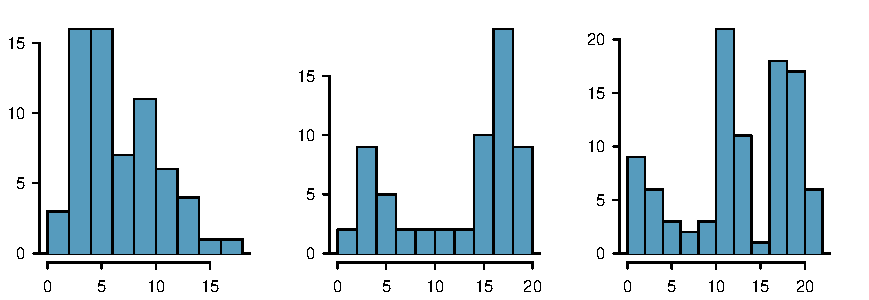
\includegraphics[width=\textwidth]{ch_intro_to_data_oi_biostat/figures/singleBiMultiModalPlots/singleBiMultiModalPlots}
	\caption{From left to right: unimodal, bimodal, and multimodal distributions.}
	\label{singleBiMultiModalPlots}
\end{figure}

\begin{exercise}
	Describe the distribution of \var{clutch.volume} using the histogram in Figure~\ref{frogHist}. Are the data skewed? Is it a unimodal, bimodal, or multimodal distribution? \footnote{The data is strongly skewed to the right; while many counts fall in the 600-1,000 $\textrm {mm}^{3}$ range, there are a few clutches with volume greater than 1,500 $\textrm {mm}^{3}$. The distribution is unimodal, with only one prominent peak.}
\end{exercise}


A \term{boxplot} summarizes a dataset using five statistics while also plotting unusual observations.\footnote{Boxplots are also known as box-and-whisker plots.} Figure~\ref{frogBoxPlot} provides a vertical dot plot alongside a boxplot of the \var{clutch.volume} variable from the \data{frog} dataset. 

\begin{figure}[th]
	\centering
	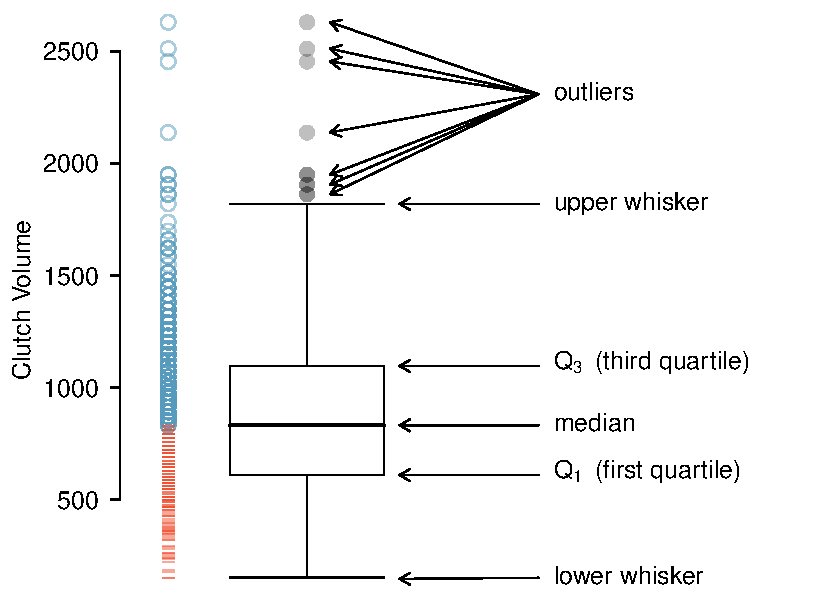
\includegraphics[width=0.86\mycaptionwidth]{ch_intro_to_data_oi_biostat/figures/frogBoxPlot/frogBoxPlot}
	\caption{A vertical dot plot next to a labeled boxplot for the volumes of 431 egg clutches. The median (831.8 $\textrm {mm}^{3}$), splits the data into the bottom 50\% and the top 50\%, marked in the dot plot by horizontal dashes and open circles, respectively.}
	\label{frogBoxPlot}
\end{figure}

In a boxplot, a rectangle extending from the first quartile to the third quartile represents the middle 50\% of the data (the IQR). The rectangle is split by the \term{median}; in an asymmetric distribution, the median need not be halfway between the first and third quartile. Extending outwards from the box, the \term{whiskers} capture the data that fall between $Q_1 - 1.5\times IQR$ and $Q_3 + 1.5\times IQR$.\footnote{While the choice of 1.5 is arbitrary, it is a commonly used value for drawing boxplots.} Note that the whiskers must end at data points; the values given by adding or subtracting $1.5\times IQR$ define the maximum reach of the whiskers. For example, for the \var{clutch.volume} variable: $Q_3 + 1.5\times IQR = 1,096.5 - 1.5\times 486.4 = 1,826.1\ \textrm {mm}^{3}$. However, there was no clutch with volume 1,826.1\ $\textrm {mm}^{3}$; thus, the upper whisker extends to 1,819.7 $\textrm {mm}^{3}$, the largest observation that is smaller than $Q_3 + 1.5\times IQR$.

Any observation that lies beyond the whiskers is shown with a dot; these observations are called outliers. An \term{outlier} is a value that appears extreme relative to the rest of the data. For the \var{clutch.volume} variable, there are several large outliers and no small outliers, indicating the presence of some unusually large egg clutches. Outliers can provide insight into interesting features of the data. 

\subsection{Scatterplots}
\label{scatterPlots}

A \term{scatterplot} provides a case-by-case view of data for two numerical variables. In the \data{frog} data, \var{clutch.volume} and \var{body.size} are two numerical variables of interest; previous research has reported that larger body size allows females to produce larger egg clutches. The relationship between clutch volume and female body size is examined via scatterplot in Figure~\ref{frogClutchVolBodySize}. In any scatterplot, each point represents a single case. Since body size was measured for 129 frogs, there are 129 points in Figure~\ref{frogClutchVolBodySize}.

The variables \var{clutch.volume} and \var{body.size} are said to be \term{associated} because the plot shows a discernible pattern. Since the points tend to lie in a straight line, the two variables are \term{linearly associated}. Two variables are \term{positively associated} if increasing values of one tend to occur with increasing values of the other; similarly, variables are \term{negatively associated} if increasing values of one variable occurs with decreasing values of the other. Figure~\ref{frogClutchVolBodySize} shows an upward trend -- as expected, larger frogs tend to produce egg clutches with larger volumes. Frog embryos are surrounded by a gelatinous matrix that may protect developing embryos from temperature fluctuation or ultraviolet radiation; these observations suggest that larger females are indeed capable of producing greater quantities of this material.

\begin{figure}
\centering
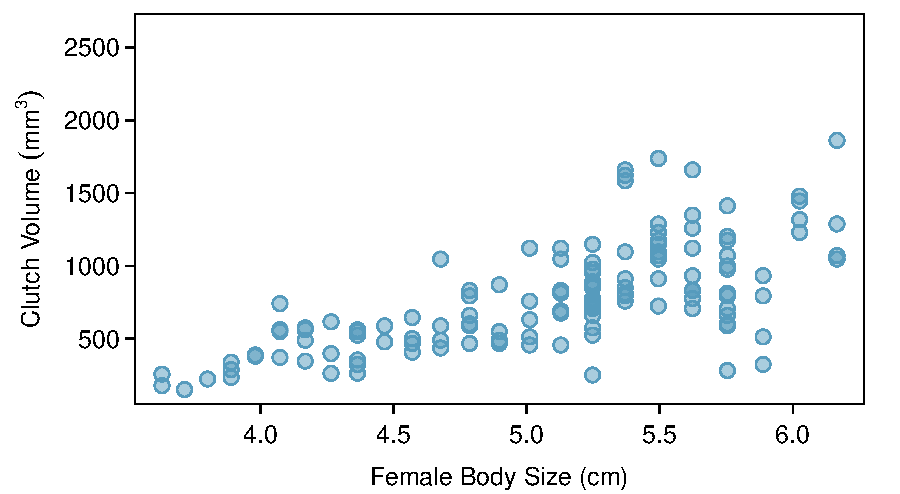
\includegraphics[width=0.8\textwidth]
{ch_intro_to_data_oi_biostat/figures/frogClutchVolBodySize/frogClutchVolBodySize}
\caption{A scatterplot showing \var{clutch.volume} (horizontal axis) vs. \var{body.size} (vertical axis). }
\label{frogClutchVolBodySize}
\end{figure}

\index{data!frog|)}
\index{data!famuss|(}

Figure~\ref{famussHeightWeight} shows the relationship between \var{height} and \var{weight} for participants in the FAMuSS study.  Each point on the plot represents a participant. As expected, taller participants tend to be heavier, so the variables \var{height} and \var{weight} are positively associated.  

\begin{figure}[h]
\centering
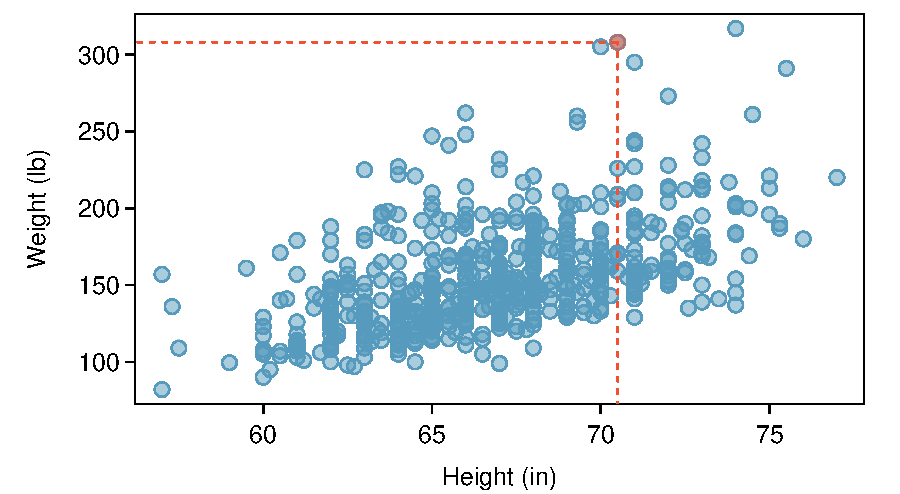
\includegraphics[width=0.8\textwidth]
{ch_intro_to_data_oi_biostat/figures/famussHeightWeight/famussHeightWeight}
\caption{A scatterplot showing \var{height} (horizontal axis) vs. \var{weight} (vertical axis). One participant 70.5 inches tall and weighing 308 pounds is highlighted.}
\label{famussHeightWeight}
\end{figure}

Taller people naturally tend to be heavier; as a consequence, weight itself is not a good measure of whether someone is overweight. Body mass index (BMI) is a measure of weight that is less affected by a person's height. A BMI of 30 or above is considered overweight.\footnote{\url{http://www.nhlbi.nih.gov/health/educational/lose_wt/risk.htm}} In the metric system, BMI is calculated as weight in kilograms (kg) divided by height squared ($\textrm {m}^{2}$). If height and weight are measured in inches and pounds, as in the \data{famuss} data, then BMI is weight in pounds (lb) divided by height squared ($\textrm {in}^{2}$), then multiplied by 703. The \data{famuss} data includes the variable \var{bmi} for each participant, and Figure~\ref{famussHeightBmi} shows the relationship between \var{height} and \var{bmi}. The strong upward trend in Figure~\ref{famussHeightWeight} is no longer evident, indicating that \var{height} and \var{bmi} have a much weaker association. For this reason, health agencies such as the US NIH and the World Health Organization (WHO) use BMI as a measure of obesity. 

\begin{figure}
\centering
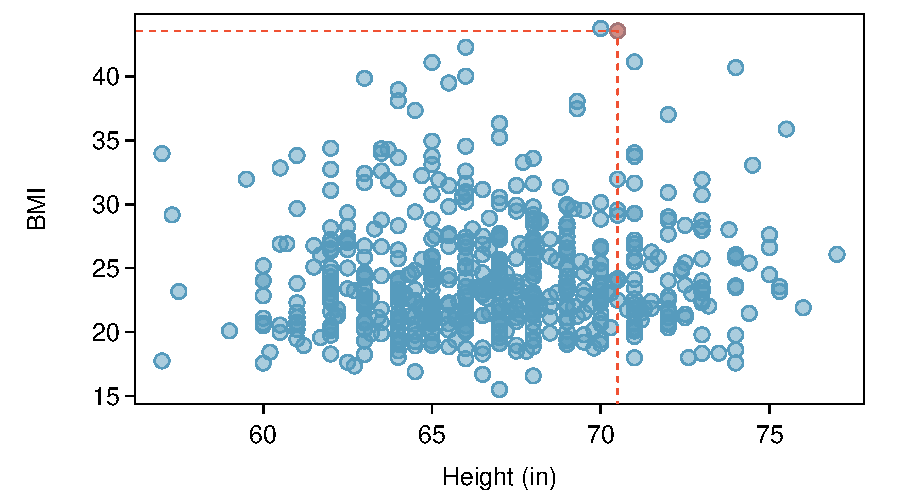
\includegraphics[width=0.8\textwidth]
{ch_intro_to_data_oi_biostat/figures/famussHeightBmi/famussHeightBmi.pdf}
\caption{A scatterplot showing \var{height} (horizontal axis) vs.  \var{bmi} (vertical axis). The same individual highlighted in Figure~\ref{famussHeightWeight} is marked here, with BMI 43.56.} 
\label{famussHeightBmi}
\end{figure}


If two variables are not associated, then they are said to be \term{independent}. That is, two variables are independent if there is no evident relationship between the two.  Generally, it is not easy to determine definitively whether two variables are independent from looking at a scatterplot, even in Figure~\ref{famussHeightBmi}.

\index{data!famuss|)}

Not all associations are linear.  In fact, some can be highly nonlinear, relationships in which clearly do not scatter about a straight line.  Figure~\ref{incomeLifeExpectancy} shows the relationship between annual per capita income and life expectancy for 248 country in 2012. Income is measured in US dollars (adjusted for purchasing power in a country) and the average expected life for children born in 2012.   The figure shows clearly that small when income is low, small increases in per capita income are associated with relatively large changes in life expectancy.  When per capita income exceeds approximately \$20,000 per year, increases in income are associated with smaller gains in life expectancy.


\begin{figure}
\centering
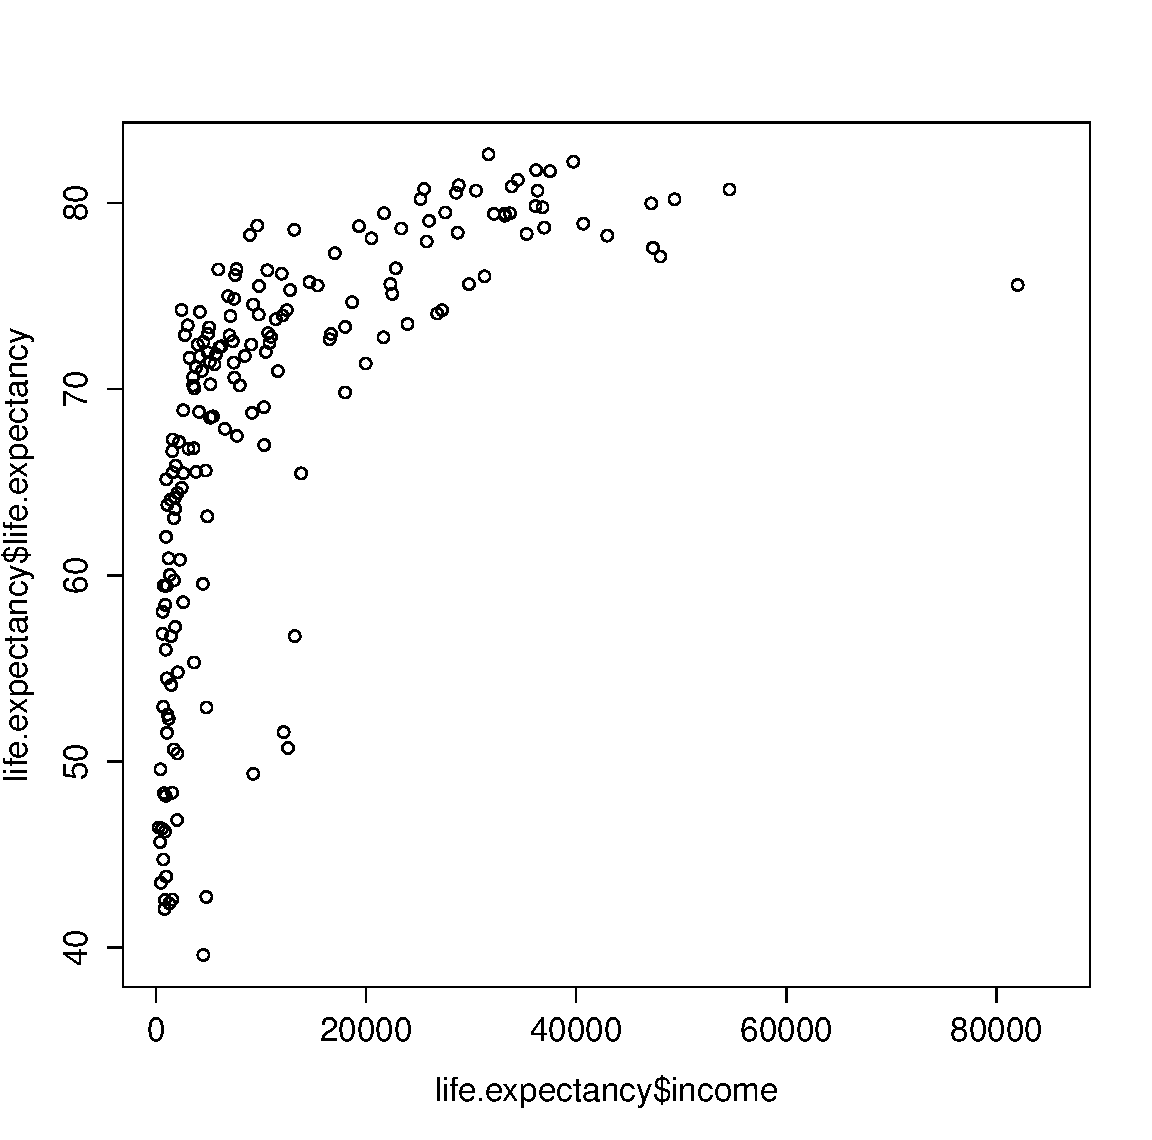
\includegraphics[width=0.8\textwidth]
{ch_intro_to_data_oi_biostat/figures/incomeLifeExpectancy/incomeLifeExpectancy.pdf}
\caption{A scatterplot showing \var{income} (horizontal axis) vs.  \var{life.expectancy} (vertical axis).} 
\label{incomeLifeExpectancy}
\end{figure}

\textit{JV: if we keep this example, the plot will have to be formatted and I should add the country to the data set.  I have more information in older stat 100 files}


\subsection{Transforming data (special topic)}
\label{transformingDataSubsection}

\index{data!frog|(}


Scientists sometimes transform strongly skewed data for several reasons. A \term{transformation} is a rescaling of the data using a function.  When the values of a variable are clustered near zero (relative to the larger values in the data set) and all observations are positive, a natural log transformation can clarify the features of a variable or the nature of a relationship\footnote{In statistics, the natural logarithm is usually written $\log$. In other settings it is sometimes written as  $\ln$.}. 

Income data are often skewed right, when measured either at the individual level or by country.  Typically, there are large clusters of low to moderate income, and a few large incomes that are outliers. The histogram of per capita incomes used for the horizontal axis in figure~\ref{incomeLifeExpectancy} is shown in Figure~\ref{incomeHistReg}. In the original scale, mean \var{income} is 14,428 (\$14,428 in US dollars) and with standard deviation \$16,391.  The empirical rule could not be used with the data on this scale, because even 1 standard deviation below the mean drops below 0. Figure~\ref{incomeHistLog} shows a plot of the $\log$ of per capita income. The $\log$ transformed data is more nearly symmetric. When a transformation has induced approximate symmetry, the empirical rule can be used to make approximate statements about the location of the transformed data, which can then be transformed back to the original scale.  On the $\log$ transformed scale, the mean $\log(income)$ is 8.86, with standard deviation 1.33.

\textit{expand on this by showing empirical rule in a plot (possibly), and calculating the middle 95\% of the log income, then transforming back to original scale.  I have added the empirical rule earlier in the chapter, but without a figure}

\textit{add discussion about value of the two scales}



\begin{figure}[ht]
\centering
\subfigure[]{
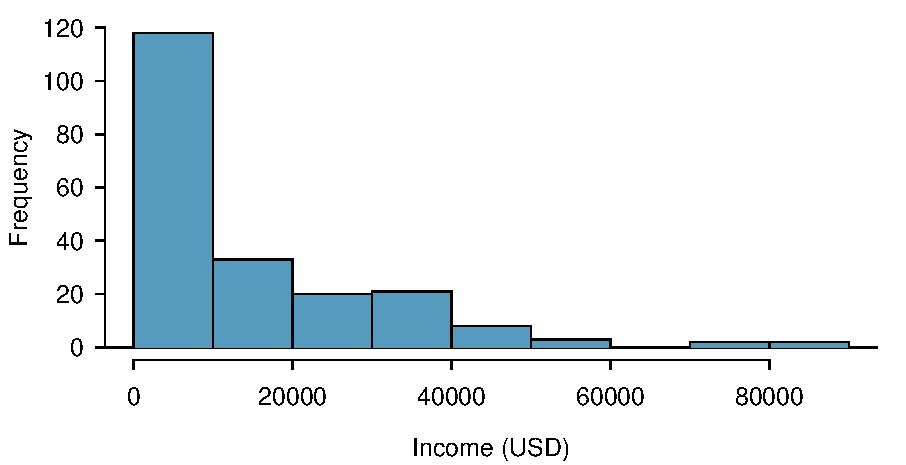
\includegraphics[width=0.46\textwidth]
{ch_intro_to_data_oi_biostat/figures/incomeHistTransformed/incomeHistReg}
\label{incomeHistReg}
}
\subfigure[]{
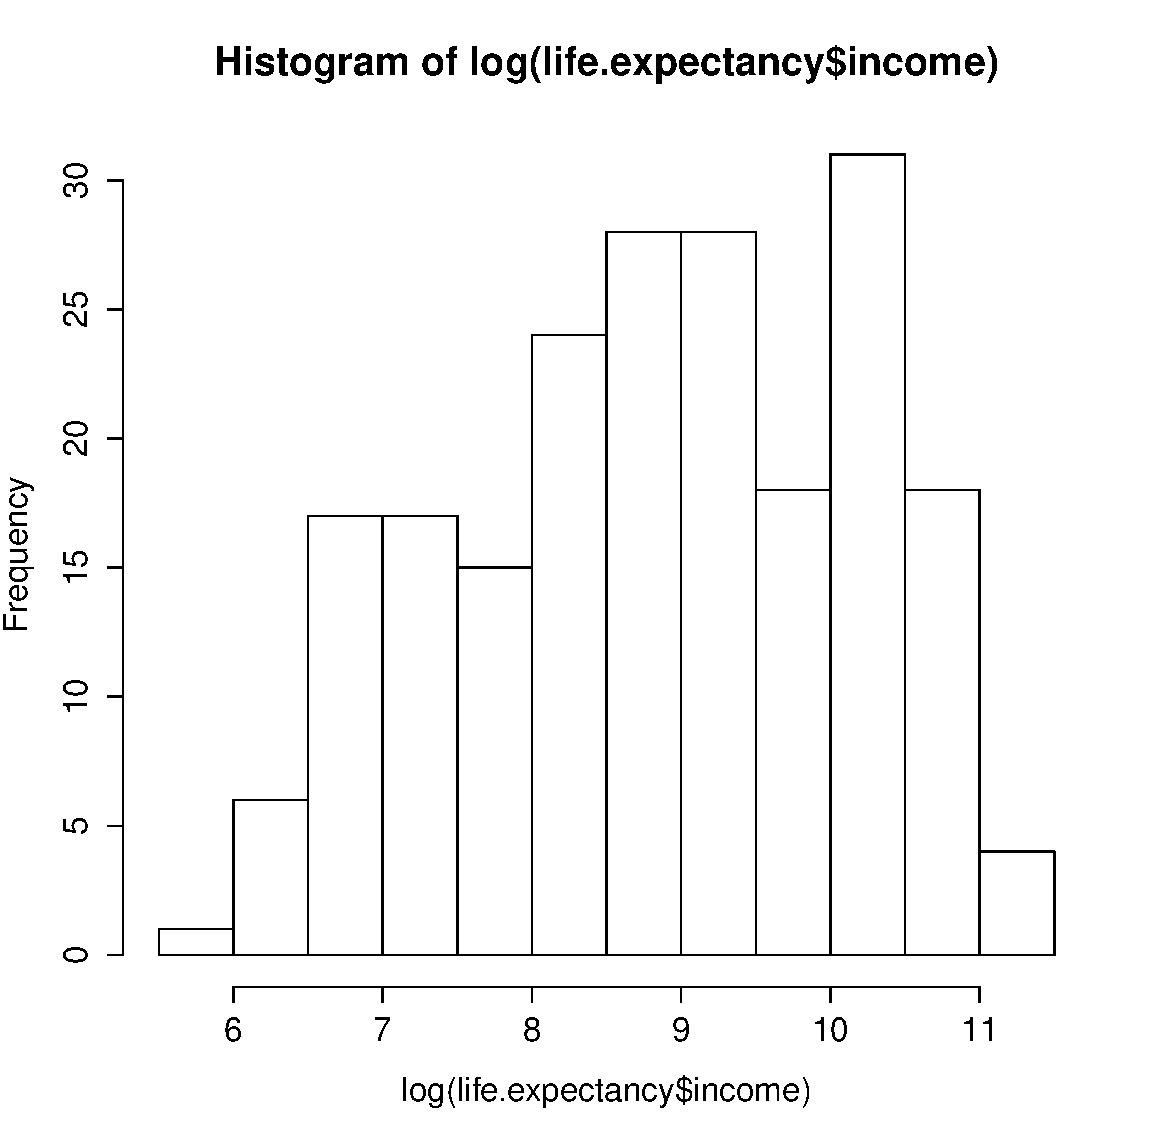
\includegraphics[width=0.46\textwidth]
{ch_intro_to_data_oi_biostat/figures/incomeHistTransformed/incomeHistLog}
\label{incomeHistLog}
}
\caption{\subref{incomeHistReg} Histogram of per capita income. \subref{incomeHistLog} Histogram of the log-transformed per capita income.}
\label{incomeHistTransform}
\end{figure}






Transformations can also used on one or both variables when exploring a relationship Figure~\ref{logIncomeLifeExpectancy} is a scatterplot of \var{log(income)} vs. \var{log(life.expectancy)}, and shows that after a log transformation for both variables, the relationship is more nearly linear.  Some statistical models are based on the assumption of an approximate linear relationship, and transformations like the log transformation will be used later when examining variables like income and life.expectancy more closely.


\begin{figure}
\centering
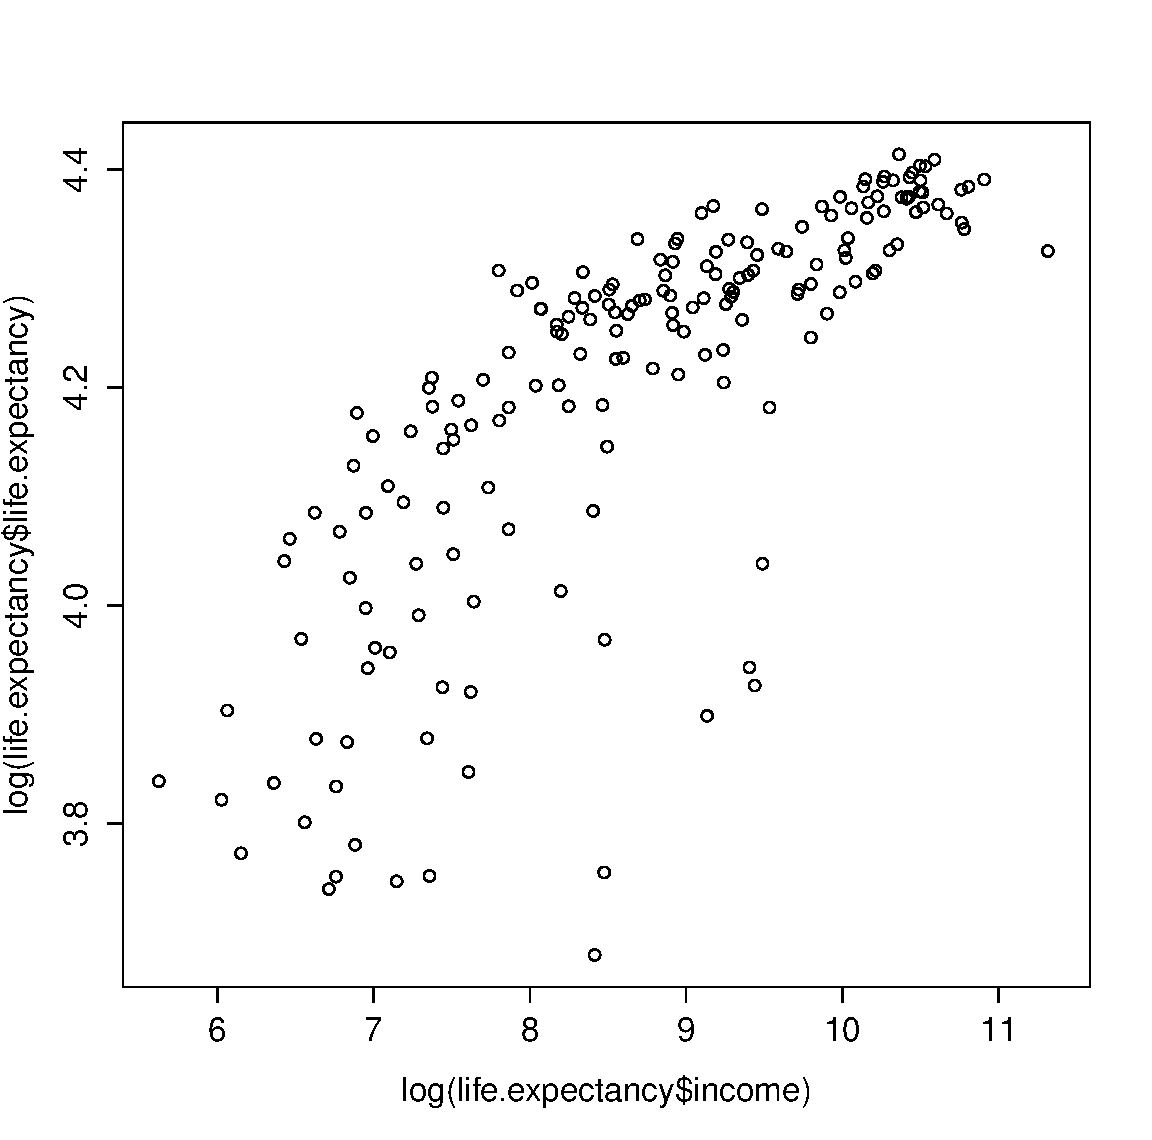
\includegraphics[width=0.8\textwidth]
{ch_intro_to_data_oi_biostat/figures/logIncomeLifeExpectancy/logIncomeLifeExpectancy.pdf}
\caption{A scatterplot showing \var{log(income)} (horizontal axis) vs.  \var{log(life.expectancy)} (vertical axis).} 
\label{logIncomeLifeExpectancy}
\end{figure}




\begin{comment}

from the JV discussion of the frog data


 A \term{transformation} is a rescaling of the data using a function. The histogram of egg clutch volumes from the \data{frog} data, shown in Figure~\ref{frogHistReg}. In the published paper, the authors used a $\textrm {log}_{10}$ transformation on the data before conducting analyses. Figure~\ref{frogHistLog} shows a plot of the $\textrm {log}_{10}$ of clutch volumes.

\begin{figure}[ht]
\centering
\subfigure[]{
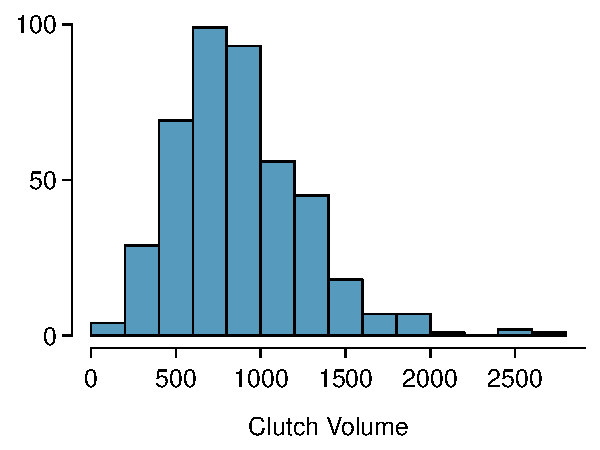
\includegraphics[width=0.46\textwidth]{ch_intro_to_data_oi_biostat/figures/frogHistTransformed/frogHistReg}
\label{frogHistReg}
}
\subfigure[]{
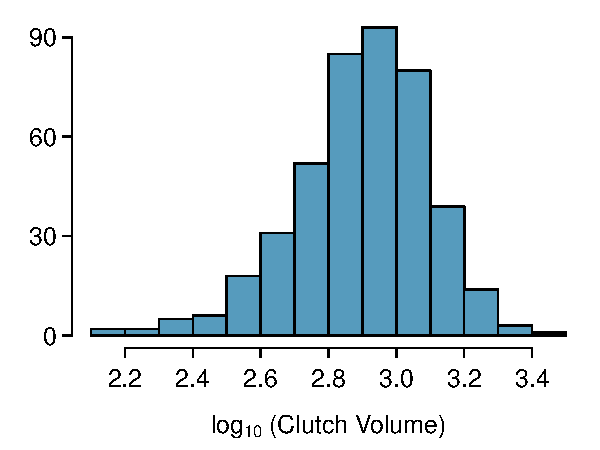
\includegraphics[width=0.46\textwidth]{ch_intro_to_data_oi_biostat/figures/frogHistTransformed/frogHistLog}
\label{frogHistLog}
}
\caption{\subref{frogHistReg} Histogram of egg clutch volumes. \subref{frogHistLog} Histogram of the log-transformed egg clutch volumes.}
\label{frogHistTransform}
\end{figure}

\end{comment}

Transformations other than the logarithm can be useful, too. For instance, the square root ($\sqrt{\text{original observation}}$) and inverse ($\frac{1}{\text{original observation}}$) are sometimes used. Common goals in transforming data are to see the data structure differently, reduce skew, assist in modeling, or straighten a nonlinear relationship in a scatterplot.

\index{data!frog|)}

\textC{\newpage}


\section[Categorical data]{Categorical data}
\label{categoricalData}

\index{data!famuss|(}

Like numerical data, categorical data can also be organized and analyzed; however, numerical calculations cannot be done with categorical data. This section introduces tables and other basic tools for categorical data, using the \data{famuss} dataset introduced in Section~\ref{variableTypes}. 

\subsection{Contingency tables}
A table for a single variable is called a \term{frequency table}. Table \ref{famussFrequencyTable} is a frequency table for the \var{actn3.r577x} variable. Recall that \var{actn3.r577x} is a categorical variable describing genotype at a location on the ACTN3 gene: CC, CT, or TT. If we replaced the counts with percentages or proportions, the table would be called a \term{relative frequency table}.

% latex table generated in R 3.0.2 by xtable 1.7-4 package
% Mon Aug 10 15:53:11 2015
\begin{table}[ht]
	\centering
	\begin{tabular}{rrrrr}
		\hline
		& CC & CT & TT & Sum \\ 
		\hline
		Counts & 173 & 261 & 161 & 595 \\ 
		\hline
	\end{tabular}
	\caption{A frequency table for the \var{actn3.r577x} variable.} 
	\label{famussFrequencyTable}
\end{table}
%library(openintro); library(xtable); data(famuss); a = addmargins(table(famuss$actn3.r577x)); genotype.table = matrix(a, ncol=4, byrow=T); colnames(genotype.table) = c("CC", "CT", "TT", "Sum"); rownames(genotype.table) = "Counts"; xtable(genotype.table, digits = 0, caption = "A frequency table for the actn3.r577x variable.", label = "famussFrequencyTable")

%JV: There is probably a cleaner way to generate this table, but wasn't sure how... OI version is below.

\begin{comment}
\begin{table}[htb]
	\centering
	\begin{tabular}{cccc}
		\hline
		none & small & big & Total \\ 
		% \hline
		549 & 2827 & 545 & 3921 \\
		\hline
	\end{tabular}
	\caption{A frequency table for the \var{number} variable.}
	\label{emailNumberTable}
\end{table}
%library(openintro); library(xtable); data(email); xtable(table(email[,c("html")]))
\end{comment}

Table \ref{famussContingencyTable} summarizes two variables: \var{race} and \var{actn3.r577x}. A table summarizing data for two categorical variables is called a \term{contingency table}.\footnote{Contingency tables are also known as \term{two-way tables}.} Each value in the table represents the number of times a particular combination of variable outcomes occurred. For example, the first row of the table shows that of the African-American individuals, 16 are CC, 6 are CT, and 5 are TT. 

Row and column totals, known collectively as \term{marginal totals}, are also included. The \term{row totals} provide the total counts across each row; \term{column totals} are the total counts down each column.

% latex table generated in R 3.0.2 by xtable 1.7-4 package
% Fri Aug 07 11:43:29 2015
\begin{table}[ht]
	\centering
	\begin{tabular}{rrrrr}
		\hline
		& CC & CT & TT & Sum \\ 
		\hline
		African Am & 16 & 6 & 5 & 27 \\ 
		Asian & 21 & 18 & 16 & 55 \\ 
		Caucasian & 125 & 216 & 126 & 467 \\ 
		Hispanic & 4 & 10 & 9 & 23 \\ 
		Other & 7 & 11 & 5 & 23 \\ 
		Sum & 173 & 261 & 161 & 595 \\ 
		\hline
	\end{tabular}
	\caption{A contingency table for \var{race} and \var{actn3.r577x}.} 
	\label{famussContingencyTable}
\end{table}
%library(xtable); data(famuss); genotype.by.race.table = addmargins(table(famuss$race, famuss$actn3.r577x)); xtable(genotype.by.race.table, digits = 0, caption = "A contingency table for race and actn3.r577x.", label = "famussContingencyTable")

\textit{JV: Not sure how they added the variable labels to their table. I have left the OI tables and code in the source.  DH: look at their source.  The created a table first (called tab) that added the var names, then applied xtable to that.  I can do it later if you like}

\begin{comment}
\begin{table}[ht]
\centering
\begin{tabular}{ll  ccc  rr}
& & \multicolumn{3}{c}{\bf \var{number}} & \\
  \cline{3-5}
& & none & small & big & Total & \hspace{2mm}\  \\ 
  \cline{2-6}
	 & spam &  149 & 168 &  50 & 367 \\ 
\raisebox{1.5ex}[0pt]{\var{spam}} 
	& not spam &  400 & 2659 & 495 & 3554 \\ 
  \cline{2-6}
& Total & 549 & 2827 & 545 & 3921 \\
  \cline{2-6}
\end{tabular}
\caption{A contingency table for \var{spam} and \var{number}.}
\label{emailSpamNumberTableTotals}
%library(openintro); library(xtable); data(email); tab <- table(email[,c("spam", "number")])[2:1,]; xtable(tab); rowSums(tab); colSums(tab); sum(tab)
\end{table}
\end{comment}

Table~\ref{famussRowPropTable} shows the row proportions for Table~\ref{famussContingencyTable}. The \termsub{row proportions}{contingency table!row proportions} are computed as the counts divided by their row totals. The value 16 at the intersection of \resp{African American} and \resp{CC} is replaced by $16/27=0.593$; i.e., 16 divided by the row total, 27. The value 0.593 corresponds to the proportion of African-Americans in the study with genotype CC.

% latex table generated in R 3.0.2 by xtable 1.7-4 package
% Fri Aug 07 11:46:57 2015
\begin{table}[ht]
	\centering
	\begin{tabular}{rrrrr}
		\hline
		& CC & CT & TT & Sum \\ 
		\hline
		African Am & $16/27=0.593$ & $6/27=0.222$ & $5/27=0.185$ & $27/27=1.00$ \\ 
		Asian & $21/55=0.382$ & $18/55=0.327$ & $16/55=0.291$ & $55/44=1.00$ \\ 
		Caucasian & $125/467=0.267$ & $216/467=0.463$ & $126/467=0.270$ & $467/467=1.00$ \\ 
		Hispanic & $4/23=0.174$ & $10/23=0.435$ & $9/23=0.391$ & $23/23=1.00$ \\ 
		Other & $7/23=0.304$ & $11/23=0.478$ & $5/23=0.217$ & $23/23=1.00$ \\ 
		Sum & $173/595=0.291$ & $261/595=0.438$ & $161/595=0.271$ & $595/595=1.00$ \\ 
		\hline
	\end{tabular}
	\caption{A contingency table with row proportions for the \var{race} and \var{actn3.r577x} variables.} 
	\label{famussRowPropTable}
\end{table}
%library(xtable); data(famuss); row.prop.table = table(famuss$race, famuss$actn3.r577x)[1:5,]; row.prop.table / rep(rowSums(row.prop.table), 3); rowSums(row.prop.table); xtable(genotype.by.race.table, digits = 0, caption = "A contingency table with row proportions for the race and actn3.r577x variables.", label = "famussRowPropTable"); 173/595; 261/595; 161/595

\begin{comment}
\begin{table}
\centering
\begin{tabular}{l rrr r}
  \hline
 & none & small & big & Total \\ 
  \hline
spam &  $149/367 = 0.406$ & $168/367 = 0.458$ &
			$50/367 = 0.136$ & 1.000 \\ 
not spam &  $400/3554 = 0.113$ & $2657/3554 = 0.748$ &
			$495/3554 = 0.139$ & 1.000 \\ 
   \hline
Total & $549/3921 = 0.140$ & $2827/3921 = 0.721$ &
			$545/3921 = 0.139$ & 1.000 \\
  \hline
\end{tabular}
\caption{A contingency table with row proportions for the \var{spam} and \var{number} variables.}
\label{rowPropSpamNumber}
% library(openintro); data(email); g <- table(email$spam, email$number)[2:1,]; g / rep(rowSums(g), 3); rowSums(g)
\end{table}
\end{comment}

\begin{example}{What does Table~\ref{famussRowPropTable} highlight about the distribution of genotypes between different populations?} 
Genotype distributions vary between populations. For the Caucasian individuals sampled in the study, CT is the most common genotype at 46.3\%. In contrast, over half (59.3\%) of African Americans sampled are CC. CC is also the most common genotype for Asians, but in this population, genotypes are more evenly distributed: 38.2\% of Asians sampled are CC, 32.7\% are CT, and 29.1\% are TT.
\end{example}

A contingency table of the column proportions is computed in a similar way, in which each \termsub{column proportion}{contingency table!column proportion} is computed as the count divided by the corresponding column total. Table~\ref{famussColPropTable} shows such a table, and here the value 0.092 indicates that 9.2\% of CC individuals in the study are African-American.

% latex table generated in R 3.0.2 by xtable 1.7-4 package
% Fri Aug 07 12:13:27 2015
\begin{table}[ht]
	\centering
	\begin{tabular}{rrrrr}
		\hline
		& CC & CT & TT & Sum \\ 
		\hline
		African Am & $16/173=0.092$ & $6/261=0.037$ & $5/161=0.191$ & $27/595=0.045$ \\ 
		Asian & $21/173=0.080$ & $18/261=0.104$ & $16/161=0.993$ & $55/595=0.092$ \\ 
		Caucasian & $125/173=0.776$ & $216/261=0.828$ & $126/161=0.728$ & $467/595=0.785$ \\ 
		Hispanic & $4/173=0.023$ & $10/261=0.062$ & $9/161=0.034$ & $23/595=0.038$ \\ 
		Other & $7/173=0.027$ & $11/261=0.063$ & $5/161=0.031$ & $23/595=0.038$ \\ 
		Sum & $173/173=1.000$ & $261/261=1.000$ & $161/161=1.000$ & $595/595=1.000$ \\ 
		\hline
	\end{tabular}
	\caption{A contingency table with column proportions for the \var{race} and \var{actn3.r577x} variables.} 
	\label{famussColPropTable}
\end{table}
%library(xtable); data(famuss); col.prop.table = table(famuss$race, famuss$actn3.r577x)[1:5,]; col.prop.table / rep(colSums(col.prop.table), 3); colSums(col.prop.table); xtable(genotype.by.race.table, digits = 0, caption = "A contingency table with column proportions for the race and actn3.r577x variables.", label = "famussColPropTable"); 27/595; 55/595; 467/595; 23/595; 23/595

\textit{JV: Not sure if the following exercise is very clear, but there should be something here to warn against misinterpretation of the column proportions in this context. Important to point out that one limitation of the data is uneven representation between groups.}

\begin{exercise}
As computed in Table~\ref{famussColPropTable}, 77.6\% of CC individuals in the study are Caucasian. Does this data suggest that in the general population, people of CC genotype are highly likely to be Caucasian?\footnote{No, this is not a reasonable conclusion to draw from the data. The high proportion of Caucasians among CC individuals primarily reflects the large number of Caucasians sampled in the study -- 78.5\% of the people sampled are Caucasian. The uneven representation of different races is one limitation of the \data{famuss} data.}
\end{exercise}

\begin{comment}
\begin{table}[h]
\centering\small
\begin{tabular}{l rrr r}
  \hline
 & none & small & big & Total \\ 
  \hline
spam &  $149/549 = 0.271$ & $168/2827 = 0.059$ &
				$50/545 = 0.092$ & $367/3921 = 0.094$ \\ 
not spam &  $400/549 = 0.729$ & $2659/2827 = 0.941$ &
				$495/545 = 0.908$ & $3684/3921 = 0.906$ \\ 
   \hline
Total & 1.000 & 1.000 & 1.000 & 1.000 \\
   \hline
\end{tabular}
\caption{A contingency table with column proportions for the \var{spam} and \var{number} variables.}
\label{colPropSpamNumber}
% library(openintro); data(email); g <- table(email$spam, email$number)[2:1,]; g / rep(colSums(g), rep(2, 3)); g; colSums(g)
\end{table}
\end{comment}

\begin{comment}
We could also have checked for an association between \var{spam} and \var{number} in Table~\ref{rowPropSpamNumber} using row proportions. When comparing these row proportions, we would look down columns to see if the fraction of emails with no numbers, small numbers, and big numbers varied from \resp{spam} to \resp{not~spam}.

\begin{exercise}
What does 0.458 represent in Table~\ref{rowPropSpamNumber}? What does 0.059 represent in Table~\ref{colPropSpamNumber}?\footnote{0.458 represents the proportion of spam emails that had a small number. 0.059 represents the fraction of emails with small numbers that are spam.}
\end{exercise}

\begin{exercise}
What does 0.139 at the intersection of \resp{not~spam} and \resp{big} represent in Table~\ref{rowPropSpamNumber}? What does 0.908 represent in the Table~\ref{colPropSpamNumber}?\footnote{0.139 represents the fraction of non-spam email that had a big number. 0.908 represents the fraction of emails with big numbers that are non-spam emails.}
\end{exercise}

\begin{example}{Data scientists use statistics to filter spam from incoming email messages. By noting specific characteristics of an email, a data scientist may be able to classify some emails as spam or not spam with high accuracy. One of those characteristics is whether the email contains no numbers, small numbers, or big numbers. Another characteristic is whether or not an email has any HTML content. A contingency table for the \var{spam} and \var{format} variables from the \data{email} data set are shown in Table~\ref{emailSpamHTMLTableTotals}. Recall that an HTML email is an email with the capacity for special formatting, e.g. bold text. In Table~\ref{emailSpamHTMLTableTotals}, which would be more helpful to someone hoping to classify email as spam or regular email: row or column proportions?} \label{weighingRowColumnProportions}
Such a person would be interested in how the proportion of spam changes within each email format. This corresponds to column proportions: the proportion of spam in plain text emails and the proportion of spam in HTML emails.

If we generate the column proportions, we can see that a higher fraction of plain text emails are spam ($209/1195 = 17.5\%$) than compared to HTML emails ($158/2726 = 5.8\%$). This information on its own is insufficient to classify an email as spam or not spam, as over 80\% of plain text emails are not spam. Yet, when we carefully combine this information with many other characteristics, such as \var{number} and other variables, we stand a reasonable chance of being able to classify some email as spam or not spam. \GLMSection{This is a topic we will return to in Chapter~\ref{multipleRegressionAndANOVA}.}{}
\end{example}

\begin{table}[ht]
\centering
\begin{tabular}{l cc r}
  \hline
 & text & HTML & Total \\ 
  \hline
spam & 209 & 158 & 367 \\ 
not spam & 986 & 2568 & 3554 \\ 
   \hline
Total & 1195 & 2726 & 3921 \\
   \hline
\end{tabular}
\caption{A contingency table for \var{spam} and \var{format}.}
\label{emailSpamHTMLTableTotals}
%library(openintro); library(xtable); data(email); tab <- table(email[,c("spam", "format")])[2:1,]; tab; colSums(tab); rowSums(tab)
\end{table}

Example~\ref{weighingRowColumnProportions} points out that row and column proportions are not equivalent. Before settling on one form for a table, it is important to consider each to ensure that the most useful table is constructed.

\begin{exercise}
Look back to Tables~\ref{rowPropSpamNumber} and~\ref{colPropSpamNumber}. Which would be more useful to someone hoping to identify spam emails using the \var{number} variable?\footnote{The column proportions in Table~\ref{colPropSpamNumber} will probably be most useful, which makes it easier to see that emails with small numbers are spam about 5.9\% of the time (relatively rare). We would also see that about 27.1\% of emails with no numbers are spam, and 9.2\% of emails with big numbers are spam.}
\end{exercise}
\end{comment}

\subsection{Bar plots}
\begin{figure}[h!]
	\centering
	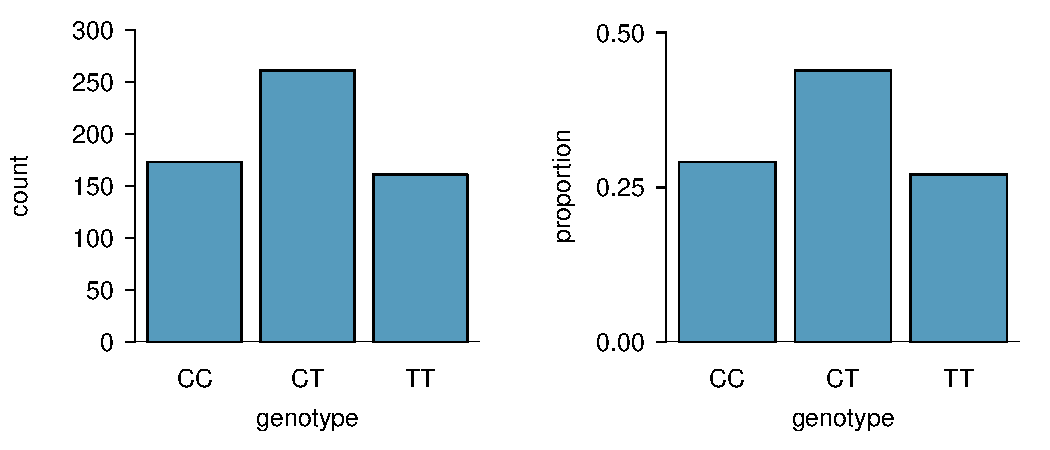
\includegraphics[width=0.9\textwidth]{ch_intro_to_data_oi_biostat/figures/famussBarPlot/famussBarPlot}
	\caption{Two bar plots of \var{actn3.r577x}. The left panel shows the counts, and the right panel shows the proportions for each genotype.}
	\label{famussBarPlot}
\end{figure}

A bar plot is a common way to display a single categorical variable. The left panel of Figure~\ref{famussBarPlot} shows a \term{bar plot} for the \var{actn3.r577x} variable. In the right panel, the counts are converted into proportions (e.g. $173/595=0.291$ for the \resp{CC} genotype), showing the proportion of observations that are in each level (i.e. in each category).

Segmented bar plots provide a way to visualize the information in contingency tables. A \termsub{segmented bar plot}{bar plot!segmented bar plot} is a graphical display of contingency table information. For example, a segmented bar plot using data from Table~\ref{famussContingencyTable} is shown in Figure~\ref{famussSegBarPlotA}, in which a bar plot was created using the \var{actn3.r577x} variable, with each group divided by the levels of \var{race}. The row proportions shown in Table~\ref{famussRowPropTable} have been translated into a standardized segmented bar plot in Figure~\ref{famussSegBarStaA}, which is a helpful visualization of the races represented in each level of \var{actn3.r577x}.

\begin{figure}[h!]
	\centering
	\subfigure[]{
		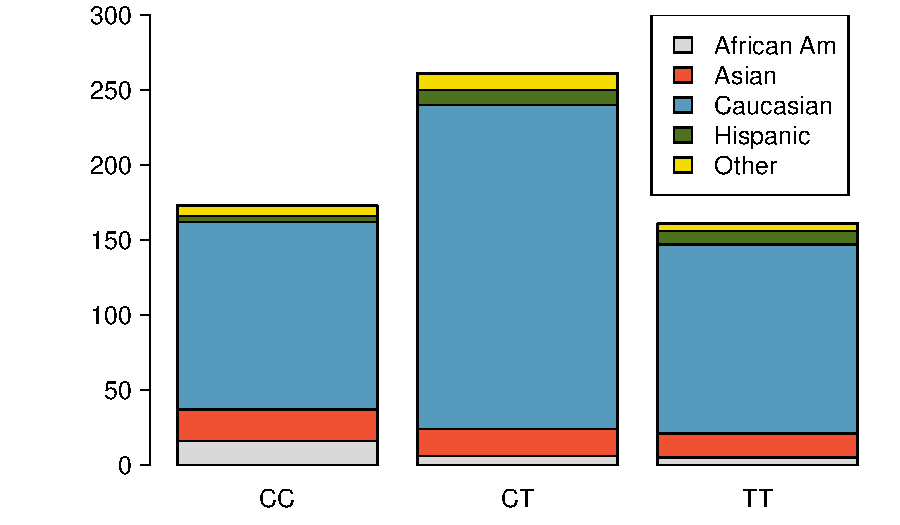
\includegraphics[width=0.46\textwidth]{ch_intro_to_data_oi_biostat/figures/famussSegBar/famussSegBarA}
		\label{famussSegBarA}
	}
	\subfigure[]{
		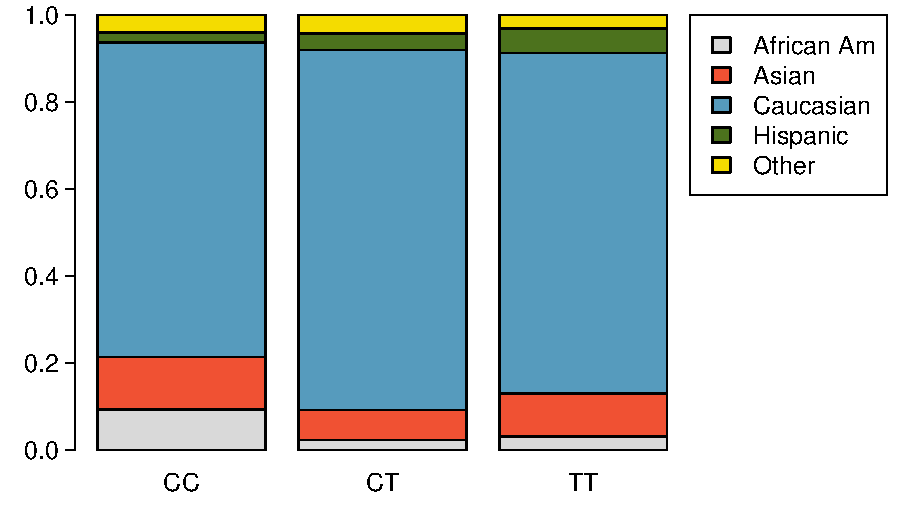
\includegraphics[width=0.46\textwidth]{ch_intro_to_data_oi_biostat/figures/famussSegBar/famussSegBarStaA} 
		\label{famussSegBarStaA}		
	}
	\caption{\subref{famussSegBarA} Segmented bar plot for individuals by genotype, where the counts have been further broken down by \var{race}. \subref{famussSegBarStaA} Standardized version of Figure~\subref{famussSegBarA}.}
	\label{famussSegBarPlotA}
\end{figure}

Alternatively, the data from the contingency table can be organized in a different way, as shown in Figure~\ref{famussSegBarPlotB}, with each bar representing a level of \var{race}. The standardized plot is particularly useful in this case, presenting the distribution of genotypes within each race more clearly than Figure~\ref{famussSegBarB}.

\begin{figure}[h!]
\centering
\subfigure[]{
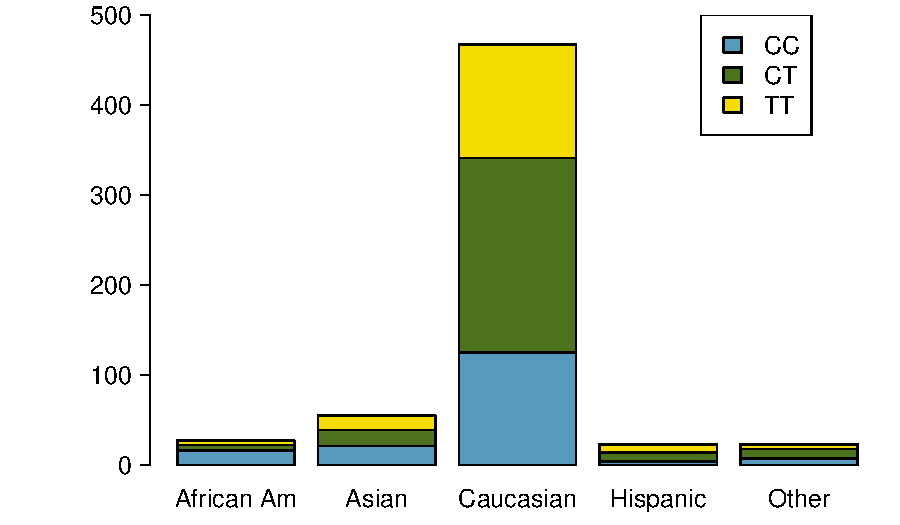
\includegraphics[width=0.46\textwidth]{ch_intro_to_data_oi_biostat/figures/famussSegBar/famussSegBarB} 
\label{famussSegBarB}
}
\subfigure[]{
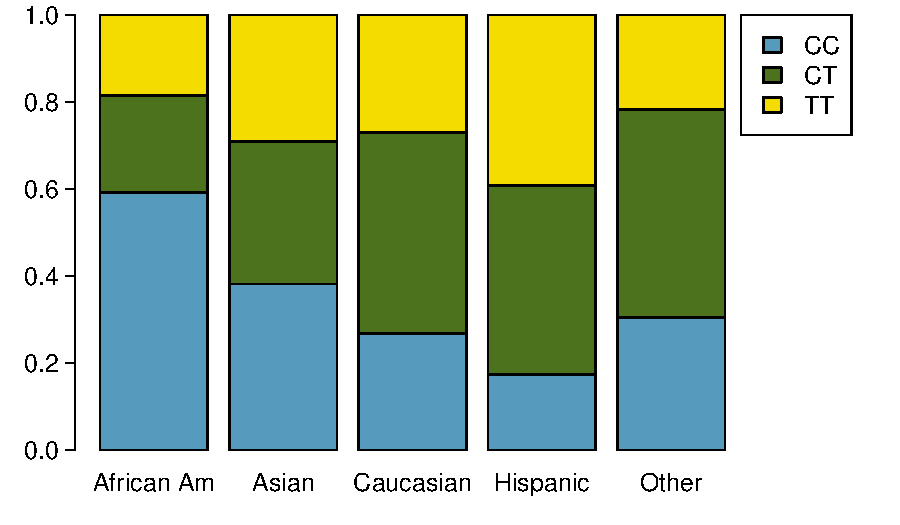
\includegraphics[width=0.46\textwidth]{ch_intro_to_data_oi_biostat/figures/famussSegBar/famussSegBarStaB} 
\label{famussSegBarStaB}	
}
\caption{\subref{famussSegBarB} Segmented bar plot for individuals by race, where the counts have been further broken down by genotype. \subref{famussSegBarStaB} Standardized version of Figure~\subref{famussSegBarB}.}
\label{famussSegBarPlotB}
\end{figure}

\begin{comment}
\begin{example}{Examine both of the segmented bar plots. Which is more useful?}
Figure~\ref{emailSpamNumberSegBar} contains more information, but Figure~\ref{emailSpamNumberSegBarSta} presents the information more clearly. This second plot makes it clear that emails with no number have a relatively high rate of spam email -- about 27\%! On the other hand, less than 10\% of email with small or big numbers are spam.
\end{example}

Since the proportion of spam changes across the groups in Figure~\ref{emailSpamNumberSegBarSta}, we can conclude the variables are dependent, which is something we were also able to discern using table proportions. Because both the \resp{none} and \resp{big} groups have relatively few observations compared to the \resp{small} group, the association is more difficult to see in Figure~\ref{emailSpamNumberSegBar}.

In some other cases, a segmented bar plot that is not standardized will be more useful in communicating important information. Before settling on a particular segmented bar plot, create standardized and non-standardized forms and decide which is more effective at communicating features of the data.
\end{comment}

\newpage
\subsection{Comparing numerical data across groups}
\label{comparingAcrossGroups}
In this section, two convenient methods for examining numerical data across groups are introduced: side-by-side boxplots and hollow histograms. The \term{side-by-side boxplot} \index{boxplot!side-by-side boxplot} is a traditional tool for comparing across categories. The \termsub{hollow histogram}{hollow histogram} method plots the outlines of histograms for each group onto the same axes.

Recall the question introduced in Section~\ref{variableRelations}: is ACTN3 genotype associated with variation in muscle function? To explore this question, genotype and variation in muscle function (measured by \var{ndrm.ch}) can be compared using side-by-side boxplots and hollow histograms, as shown in Figure~\ref{famussGenoMuscFunc}. The histograms are useful for seeing distribution shape, skew, and groups of anomalies, while the side-by-side boxplots are especially useful for comparing centers and spreads. Comparison of median change in non-dominant arm strength between the two groups reveals that the TT genotype is associated with a greater increase in strength than CC or TT. In other words, the T allele appears to be associated with greater muscle function.

\begin{figure}[h]
   \centering
   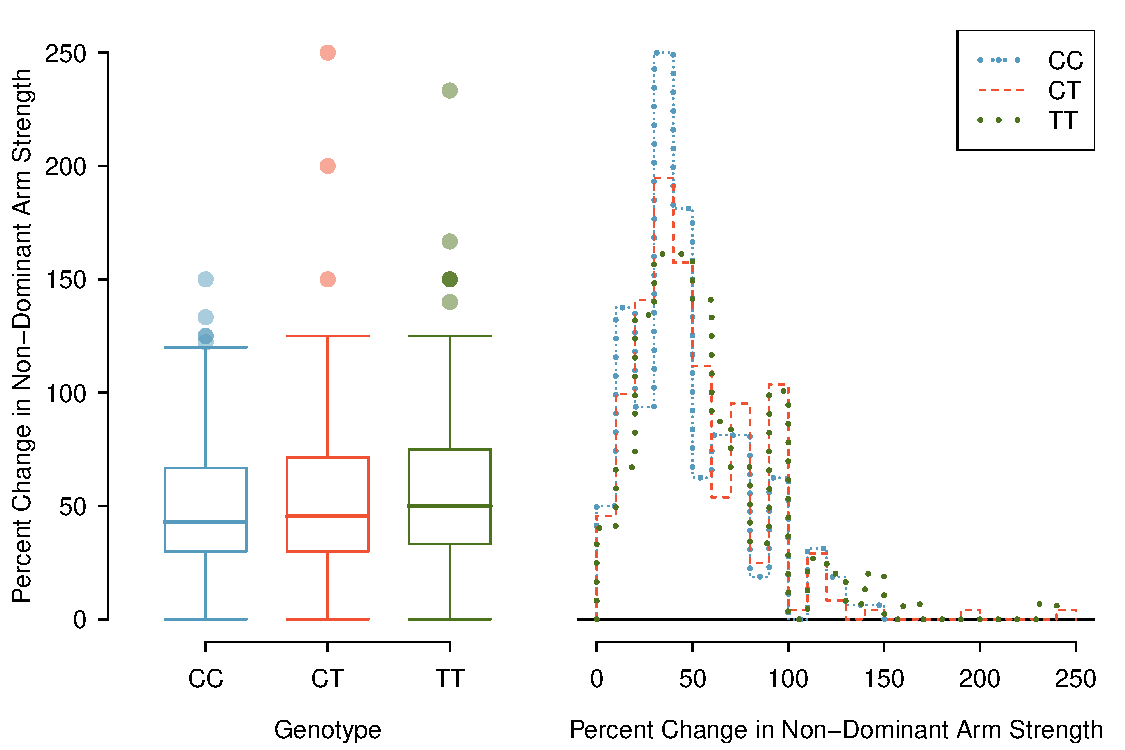
\includegraphics[width=\textwidth]{ch_intro_to_data_oi_biostat/figures/famussGenoMuscFunc/famussGenoMuscFunc}
   \caption{Side-by-side boxplot (left panel) and hollow histograms (right panel) for \var{ndrm.ch}, split by ACTN3 genotype.}
   \label{famussGenoMuscFunc}
\end{figure}

\index{data!famuss|)}

\index{data!frog|(}

Not all data will show such apparent trends. For example, consider the question of interest in the \data{frog} dataset: how does maternal investment vary with altitude? Researchers collected data at 11 altitudes from 2,035 to 3,495 m above sea level, measuring attributes of egg clutches such as clutch volume. A side-by-side boxplot comparing clutch volume across altitudes is shown in Figure~\ref{frogClutchVolAlt}. It seems that as a general rule, clutches found at higher altitudes have greater volume. However, more advanced statistical methods, such as those used in the published study, are required to thoroughly investigate the potential association between altitude and clutch size. 

\begin{figure}
	\centering
	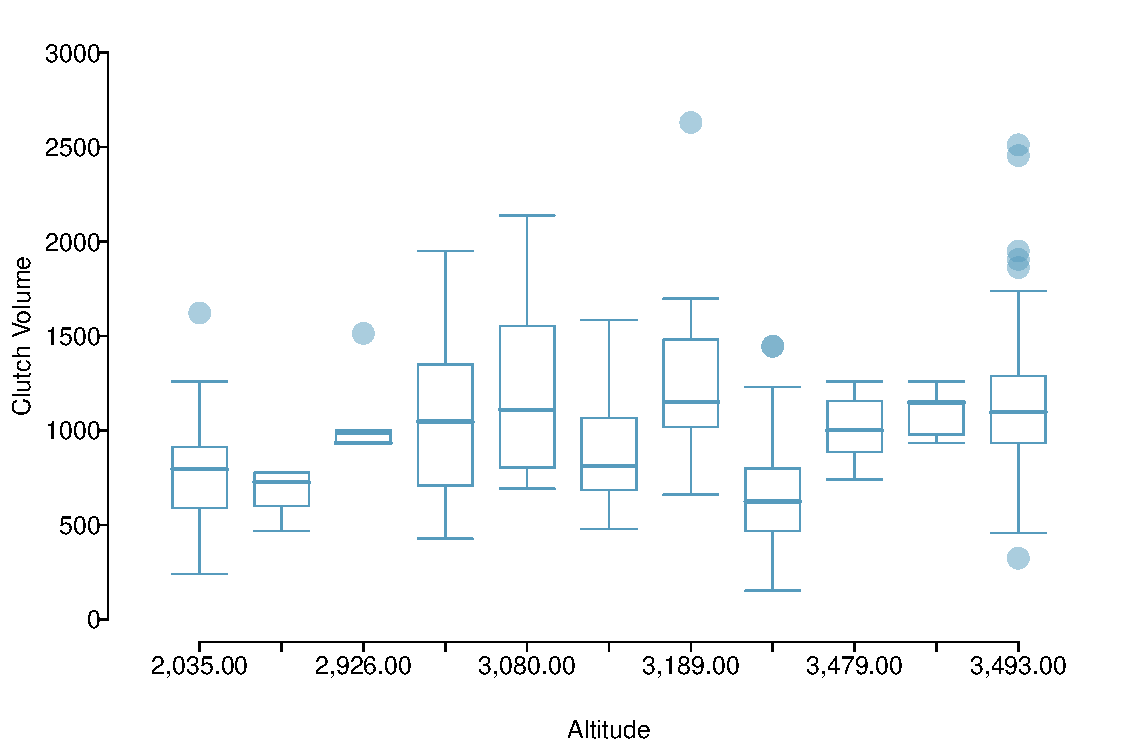
\includegraphics[width=\textwidth]{ch_intro_to_data_oi_biostat/figures/frogClutchVolAlt/frogClutchVolAlt}
	\caption{Side-by-side boxplot comparing the distribution of \var{clutch.volume} for different altitudes.}
	\label{frogClutchVolAlt}
\end{figure} 

\index{data!frog|)}

\begin{comment}
\begin{exercise} \label{comparingPriceByTypeExercise}
Use the plots in Figure~\ref{countyIncomeSplitByPopGain} to compare the incomes for counties across the two groups. What do you notice about the approximate center of each group? What do you notice about the variability between groups? Is the shape relatively consistent between groups? How many \emph{prominent} modes are there for each group?\footnote{Answers may vary a little. The counties with population gains tend to have higher income (median of about \$45,000) versus counties without a gain (median of about \$40,000). The variability is also slightly larger for the population gain group. This is evident in the IQR, which is about 50\% bigger in the \emph{gain} group. Both distributions show slight to moderate right skew\index{skew!example: slight to moderate} and are unimodal. There is a secondary small bump at about \$60,000 for the \emph{no gain} group, visible in the hollow histogram plot, that seems out of place. (Looking into the data set, we would find that 8 of these 15 counties are in Alaska and Texas.) The box plots indicate there are many observations far above the median in each group, though we should anticipate that many observations will fall beyond the whiskers when using such a large data set.}
\end{exercise}

\begin{exercise}
What components of each plot in Figure~\ref{countyIncomeSplitByPopGain} do you find most useful?\footnote{Answers will vary. The side-by-side box plots are especially useful for comparing centers and spreads, while the hollow histograms are more useful for seeing distribution shape, skew, and groups of anomalies.}
\end{exercise}
\end{comment}

\end{doublespace}

